% Options for packages loaded elsewhere
\PassOptionsToPackage{unicode}{hyperref}
\PassOptionsToPackage{hyphens}{url}
%
\documentclass[
  man,floatsintext]{apa6}
\usepackage{amsmath,amssymb}
\usepackage{iftex}
\ifPDFTeX
  \usepackage[T1]{fontenc}
  \usepackage[utf8]{inputenc}
  \usepackage{textcomp} % provide euro and other symbols
\else % if luatex or xetex
  \usepackage{unicode-math} % this also loads fontspec
  \defaultfontfeatures{Scale=MatchLowercase}
  \defaultfontfeatures[\rmfamily]{Ligatures=TeX,Scale=1}
\fi
\usepackage{lmodern}
\ifPDFTeX\else
  % xetex/luatex font selection
\fi
% Use upquote if available, for straight quotes in verbatim environments
\IfFileExists{upquote.sty}{\usepackage{upquote}}{}
\IfFileExists{microtype.sty}{% use microtype if available
  \usepackage[]{microtype}
  \UseMicrotypeSet[protrusion]{basicmath} % disable protrusion for tt fonts
}{}
\makeatletter
\@ifundefined{KOMAClassName}{% if non-KOMA class
  \IfFileExists{parskip.sty}{%
    \usepackage{parskip}
  }{% else
    \setlength{\parindent}{0pt}
    \setlength{\parskip}{6pt plus 2pt minus 1pt}}
}{% if KOMA class
  \KOMAoptions{parskip=half}}
\makeatother
\usepackage{xcolor}
\usepackage{longtable,booktabs,array}
\usepackage{calc} % for calculating minipage widths
% Correct order of tables after \paragraph or \subparagraph
\usepackage{etoolbox}
\makeatletter
\patchcmd\longtable{\par}{\if@noskipsec\mbox{}\fi\par}{}{}
\makeatother
% Allow footnotes in longtable head/foot
\IfFileExists{footnotehyper.sty}{\usepackage{footnotehyper}}{\usepackage{footnote}}
\makesavenoteenv{longtable}
\usepackage{graphicx}
\makeatletter
\def\maxwidth{\ifdim\Gin@nat@width>\linewidth\linewidth\else\Gin@nat@width\fi}
\def\maxheight{\ifdim\Gin@nat@height>\textheight\textheight\else\Gin@nat@height\fi}
\makeatother
% Scale images if necessary, so that they will not overflow the page
% margins by default, and it is still possible to overwrite the defaults
% using explicit options in \includegraphics[width, height, ...]{}
\setkeys{Gin}{width=\maxwidth,height=\maxheight,keepaspectratio}
% Set default figure placement to htbp
\makeatletter
\def\fps@figure{htbp}
\makeatother
\setlength{\emergencystretch}{3em} % prevent overfull lines
\providecommand{\tightlist}{%
  \setlength{\itemsep}{0pt}\setlength{\parskip}{0pt}}
\setcounter{secnumdepth}{-\maxdimen} % remove section numbering
% Make \paragraph and \subparagraph free-standing
\ifx\paragraph\undefined\else
  \let\oldparagraph\paragraph
  \renewcommand{\paragraph}[1]{\oldparagraph{#1}\mbox{}}
\fi
\ifx\subparagraph\undefined\else
  \let\oldsubparagraph\subparagraph
  \renewcommand{\subparagraph}[1]{\oldsubparagraph{#1}\mbox{}}
\fi
\newlength{\cslhangindent}
\setlength{\cslhangindent}{1.5em}
\newlength{\csllabelwidth}
\setlength{\csllabelwidth}{3em}
\newlength{\cslentryspacingunit} % times entry-spacing
\setlength{\cslentryspacingunit}{\parskip}
\newenvironment{CSLReferences}[2] % #1 hanging-ident, #2 entry spacing
 {% don't indent paragraphs
  \setlength{\parindent}{0pt}
  % turn on hanging indent if param 1 is 1
  \ifodd #1
  \let\oldpar\par
  \def\par{\hangindent=\cslhangindent\oldpar}
  \fi
  % set entry spacing
  \setlength{\parskip}{#2\cslentryspacingunit}
 }%
 {}
\usepackage{calc}
\newcommand{\CSLBlock}[1]{#1\hfill\break}
\newcommand{\CSLLeftMargin}[1]{\parbox[t]{\csllabelwidth}{#1}}
\newcommand{\CSLRightInline}[1]{\parbox[t]{\linewidth - \csllabelwidth}{#1}\break}
\newcommand{\CSLIndent}[1]{\hspace{\cslhangindent}#1}
\ifLuaTeX
\usepackage[bidi=basic]{babel}
\else
\usepackage[bidi=default]{babel}
\fi
\babelprovide[main,import]{english}
% get rid of language-specific shorthands (see #6817):
\let\LanguageShortHands\languageshorthands
\def\languageshorthands#1{}
% Manuscript styling
\usepackage{upgreek}
\captionsetup{font=singlespacing,justification=justified}

% Table formatting
\usepackage{longtable}
\usepackage{lscape}
% \usepackage[counterclockwise]{rotating}   % Landscape page setup for large tables
\usepackage{multirow}		% Table styling
\usepackage{tabularx}		% Control Column width
\usepackage[flushleft]{threeparttable}	% Allows for three part tables with a specified notes section
\usepackage{threeparttablex}            % Lets threeparttable work with longtable

% Create new environments so endfloat can handle them
% \newenvironment{ltable}
%   {\begin{landscape}\centering\begin{threeparttable}}
%   {\end{threeparttable}\end{landscape}}
\newenvironment{lltable}{\begin{landscape}\centering\begin{ThreePartTable}}{\end{ThreePartTable}\end{landscape}}

% Enables adjusting longtable caption width to table width
% Solution found at http://golatex.de/longtable-mit-caption-so-breit-wie-die-tabelle-t15767.html
\makeatletter
\newcommand\LastLTentrywidth{1em}
\newlength\longtablewidth
\setlength{\longtablewidth}{1in}
\newcommand{\getlongtablewidth}{\begingroup \ifcsname LT@\roman{LT@tables}\endcsname \global\longtablewidth=0pt \renewcommand{\LT@entry}[2]{\global\advance\longtablewidth by ##2\relax\gdef\LastLTentrywidth{##2}}\@nameuse{LT@\roman{LT@tables}} \fi \endgroup}

% \setlength{\parindent}{0.5in}
% \setlength{\parskip}{0pt plus 0pt minus 0pt}

% Overwrite redefinition of paragraph and subparagraph by the default LaTeX template
% See https://github.com/crsh/papaja/issues/292
\makeatletter
\renewcommand{\paragraph}{\@startsection{paragraph}{4}{\parindent}%
  {0\baselineskip \@plus 0.2ex \@minus 0.2ex}%
  {-1em}%
  {\normalfont\normalsize\bfseries\itshape\typesectitle}}

\renewcommand{\subparagraph}[1]{\@startsection{subparagraph}{5}{1em}%
  {0\baselineskip \@plus 0.2ex \@minus 0.2ex}%
  {-\z@\relax}%
  {\normalfont\normalsize\itshape\hspace{\parindent}{#1}\textit{\addperi}}{\relax}}
\makeatother

% \usepackage{etoolbox}
\makeatletter
\patchcmd{\HyOrg@maketitle}
  {\section{\normalfont\normalsize\abstractname}}
  {\section*{\normalfont\normalsize\abstractname}}
  {}{\typeout{Failed to patch abstract.}}
\patchcmd{\HyOrg@maketitle}
  {\section{\protect\normalfont{\@title}}}
  {\section*{\protect\normalfont{\@title}}}
  {}{\typeout{Failed to patch title.}}
\makeatother

\usepackage{xpatch}
\makeatletter
\xapptocmd\appendix
  {\xapptocmd\section
    {\addcontentsline{toc}{section}{\appendixname\ifoneappendix\else~\theappendix\fi\\: #1}}
    {}{\InnerPatchFailed}%
  }
{}{\PatchFailed}
\keywords{L3 acquisition, equivalence testing, replication\newline\indent Word count: 6982}
\usepackage{lineno}

\linenumbers
\usepackage{csquotes}
\ifLuaTeX
  \usepackage{selnolig}  % disable illegal ligatures
\fi
\IfFileExists{bookmark.sty}{\usepackage{bookmark}}{\usepackage{hyperref}}
\IfFileExists{xurl.sty}{\usepackage{xurl}}{} % add URL line breaks if available
\urlstyle{same}
\hypersetup{
  pdftitle={Statistical Insignificance is not wholesale transfer in L3 acquisition: An Approximate Replication of Rothman (2011)},
  pdfauthor={Kyle Parrish1},
  pdflang={en-EN},
  pdfkeywords={L3 acquisition, equivalence testing, replication},
  hidelinks,
  pdfcreator={LaTeX via pandoc}}

\title{Statistical Insignificance is not wholesale transfer in L3 acquisition: An Approximate Replication of Rothman (2011)}
\author{Kyle Parrish\textsuperscript{1}}
\date{}


\shorttitle{Rothman (2011) Replication}

\authornote{

Correspondence concerning this article should be addressed to Kyle Parrish, 15 Seminary Place, New Brunswick, NJ. E-mail: \href{mailto:kyle.parrish@rutgers.edu}{\nolinkurl{kyle.parrish@rutgers.edu}}

}

\affiliation{\vspace{0.5cm}\textsuperscript{1} Rutgers University}

\abstract{%
The present study was an approximate replication of Rothman (2011) and examined the determiner phrase (DP) syntax of a large sample (n = 211) of L3 learners of Portuguese who spoke English and Spanish.
Rothman (2011) investigated whether L3 Italian or Brazilian Portuguese speakers would be differently impacted by another known Romance Language if it was their L1 or L2.
The original study concluded that groups did not perform differently on the experimental tasks on the basis of a null effect, and that the typological similarity of Spanish and Portuguese or Italian, relative to English, predicts transfer in the initial stages of L3 acquisition.
The present replication recreated all materials, which were not available, but examined the same population and questions.
Rather than examining L3 Italian and L3 Brazilian Portuguese, the present work maintained a constant L3, Portuguese
The learners were divided into two groups in a mirror-image design (n = 96 L1 English-L2 Spanish, n = 115 L1 Spanish-L2 English) and data was collected completely online.
Like the original study, there was not a main effect of group in any of the two-way Analyses of Variance.
However, these results show that it should not be assumed that experimental groups behave equivalently based on a null effect: out of four total post-hoc tests of equivalence, only two were significant when the equivalence bounds were set at a small effect size (d = +/- .4).
Ultimately, it is argued that determining the smallest effect size of interest and subsequent equivalence testing are necessary to answer key questions in the field of L3 acquisition.
}



\begin{document}
\maketitle

\hypertarget{introduction}{%
\section{Introduction}\label{introduction}}

The field of third language acquisition is still far from agreeing upon exactly how previously known languages (the first and second learned languages) impact the initial stages of third language (L3) development.
One key debate in the field regards whether the perceived typological similarity of previously known languages drives transfer to the L3, or whether order of acquisition plays a role.
For example, there is some evidence of the second language (L2) impacting the L3 even when the L1 would be a better choice (Bardel \& Falk, 2007; Falk, 2017; Falk \& Bardel, 2011; Hopp, 2019).
This view has been formalized as the L2 Status Factor Model, which predicts that the L2 is a privileged source of transfer to the L3 based on the cognitive similarity between late-learned languages (Bardel \& Falk, 2012; Paradis, 2009).
On the other hand, a prominent model in the field, the Typological Primacy Model (TPM), posits that wholesale transfer, or the transfer of the entire L1 or L2 system (but not both) occurs.
The language to be transferred is chosen given hierarchical cues from L3 input to determine which source language (the L1 or L2) is more typologically similar to the language being learned and occurs during the initial stages of L3 development, estimated by to be some 20-30 hours of L3 instruction.
In the TPM, wholesale transfer is motivated by cognitive economy, in which it is argued that transferring two languages is more cognitively demanding than one.
This process is argued to be a cognitive reflex, in which the parser transfers one whole language at the earliest possible moment in L3 development.

The initial proposal of the Typological Primacy Model was based primarily on data published in Rothman (2011).
In the study, the determiner phrase syntax of two groups of L3 learners of Spanish or Brazilian Portuguese were tested using a Semantic Interpretation Task and a Context-Based Collocation Task.
Specifically, the study examined how pre and postnominal adjectives impacted noun meaning.
In Romance languages, but not English, a difference in meaning occurs when an adjective appears in prenominal or postnominal position.
For example, in Spanish, \emph{el viejo amigo} refers to an friend one has had for a long time, while \emph{el amigo viejo} refers to a friend who is old.
The two groups both spoke two Romance languages and English, but varied as to whether their L1 or L2 was a Romance language: the first group spoke L3 Spanish (L1 English/L2 Spanish) and the second group spoke L3 Italian (L1 Spanish/L2 English).
The results showed that, in both tasks and groups, the participants showed high levels of accuracy in their L3 determiner phrase syntax.
The analysis of the data revealed no significant effect of group in the Analysis of Variance.

One key method utilized in Rothman (2011) was the use of mirror-image like groups (Bardel \& Falk, 2007; Foote, 2009).
In a mirror image design, two groups of L3 learners (learning language A) are compared.
These groups speak the same languages, but in the opposite order (L1 language - L2 language C vs.~L1 language C - L2 language B).
This choice was made in order to rule out order of acquisition effects documented in other studies (e.g. Bardel \& Falk, 2007; Hermas, 2010, 2014), which suggest that either the L1 or L2 have a special status for transfer based on their order of having been acquired.
One objective of this design thus becomes to provide evidence that the two groups perform similarly on a given task.
If groups do perform similarly, it would provide evidence that order of acquisition does not predict whether a source language will impact the L3, and that two groups of subjects both have access to the same language during L3 learning, whether or not it is the L1 or the L2.
It is worth mentioning that, since the time of the original paper, considerable evidence has shown that order of acquisition cannot explain many outcomes observed in the L3 initial stages of morphosyntax (see Puig-Mayenco et al., 2020 for a review), and the debate has now shifted to whether structural or holistic similarity play a decisive role in transfer.

Using the mirror image design, several studies have made comparisons of two mirror image groups of L3 speakers with the goal being to demonstrate that they perform similarly on an experimental task, and, as a result, are impacted by the same source language whether it is their L1 or their L2.
In these studies, a popular statistical choice has been to use an Analysis of Variance (ANOVA), in which a given continuous outcome variable (such as percentage correct) is analyzed as a function of a categorical variable(s) (such as group).
In this analysis, the researcher typically carries out a nested model comparison to assess for main effects and interactions given a significance threshold.
The presence of a main effect or interaction with a p-value under the significance threshold has been referred to as statistically significantly different.
On the other hand, if there is no main effect during a nested model comparison, this suggests that a given predictor does not explain any additional variance in the observed data.
In much of the work done on the TPM, the lack of a main effect has been used as evidence of similar performance between groups.
For example, in the original study, Rothman (2011) concluded, on the basis of the lack of a main effect or interaction, that ``the statistical analyses presented above demonstrate that both sets of L3 learners were successful on the experiments without any statistically significant deviance from the native speaker controls. As such, it goes without saying, but is noteworthy nonetheless, that they did not differ from each other either'' (p.~120).
Other studies followed this interpretation, such as Borg (2013), who investigated the acquisition of future-tense probability in L3 Spanish by L1 English-L2 French and L1 French-L2 English speakers.
Like Rothman (2011), there was not an effect in the group comparison, and the author concluded that the two L3 groups ``..the results in this condition follow our predictions in that there is no significant difference between the two L3 groups'' (p.~17).
A similar approach was taken by Puig-Mayenco and Rothman (2020), who found that, in a subset of their data, that two distinct L3 English structures were influenced by the same source language by mirror image groups of Catalan-Spanish bilinguals on the basis of the lack of a main effect.
Some scholars, such as Lago (2021), have argued that results of the body of work for the TPM largely should be considered inconclusive, given that the lack of a main effect does not entail practical equivalence (Altman \& Bland, 1995).
Specifically, Null Hypothesis Significance Testing (NHST) does not provide evidence itself for practical equivalence, but only the ability to reject the null hypothesis (suggest that there is a difference).

It is argued in the present work that specific criteria for both the null hypothesis (that no meaningful differences exist between groups) and the alternative hypothesis (that there is some difference) should be specified to the point that it is possible prior to carrying out an experiment.
While methods for establishing statistical differences are ubiquitous, the use of statistical methods to provide evidence of the lack of a difference is less prevalent.
One method to establish equivalence is equivalence testing (Lakens et al., 2018).
Similar to a t-test, equivalence testing utilizes a significance threshold (typically .05) and equivalence bounds (ideally determined by theory and equal to the smallest effect size of interest).
The test is considered significant if the 90\% confidence interval surrounding the observed mean difference falls within the equivalence bounds.
Assuming that the standard deviation of the original study (which was not reported) is similar to the present study (1.20), the power of the original study could only reliably detect practical equivalence if the bounds were set d = +/- -1.07 at a power level of .8.
This is typically considered a very large effect.
Again assuming a similar standard deviation, this effect would correspond to a difference of approximately 0.26 in percentage correct between groups.
As such, the sample of the original study could only reliably detect equivalence if the effect was quite large.
In fact, a power analysis assuming the same standard deviation reveals that the power of a test of equivalence in original study was 0 (n = 13 per group, power level = .8, alpha = .05, equivalence bounds d = +/- .4).

It is also the case that many studies with of third languages have low sample sizes.
The impact of these low sample sizes is high uncertainty surrounding insignificant results in low sample studies.
One consequence of low statistical power is an increased false negative rate (type II error).
As the true effect size between two groups or conditions decreases, the number of observations (or participants) that are necessary to detect the effect increases.
In other words, to detect a small effect, one needs many participants.
For example, in order to detect an effect of Cohen's D = +/- .4, a power analysis reveals that 98 participants are needed to achieve a power level of .8 at the significance level of .05.

\hypertarget{motivation-for-replication}{%
\section{Motivation for Replication:}\label{motivation-for-replication}}

The present study was an approximate replication of Rothman (2011).
An approximate replication refers to no more than two variables being changed from the original study (McManus, 2022; Porte \& McManus, 2018).
Although the variables are not changed directly, the tasks used to measure them were both changed in the present study, since the original materials are no longer available.
The experiential tasks were recreated with input from the original author and on the basis of the examples provided Rothman (2011), such that the same number of stimuli were being sampled in the same conditions.
The research question, population, and original analyses were all able to be held constant.

A replication of Rothman (2011) was primarily proposed due to a combination of the sample size of the original study and the statistical tests used.
It is important to note that Rothman (2011) and several subsequent studies are quite similar in their use of statistical tests and group designs, and that any of them could logically be chosen for replication on the basis of the same logic used to select Rothman (2011).
However, it was Rothman (2011) in which the Typological Primacy Model was proposed.
The TPM has been a highly influential model and Rothman (2011) has largely influenced how subsequent studies to evaluate its claims were carried out.
In particular, a failed replication of this study could call into question each of these studies that used similar statistical methods.

Unfortunately, the stimuli from the original study were lost and as a result had to be recreated using the descriptions from the original study and an example of each task as a basis.
The stimuli were adapted from a combination of examples provided in Rothman (2011) and Judy (2021), which both reported Spanish versions of a Semantic Interpretation task and a Context-Based Collocation task.
The stimuli and answer choices were translated to Portuguese and chosen so that 10 total tokens remained with 5 preposed and 5 postposed adjectives in each task remained.
In addition to new stimuli, the groups were changed from the original study so that both groups spoke the same 3 languages.
In the original study, the two groups were L1 English - L2 Spanish - L3 Brazilian Portuguese and L1 Italian - L2 English - L3 Spanish speakers.
This group difference made it necessary to create both Spanish and Brazilian Portuguese versions of the experimental tasks.
The present study used mirror image groups of Spanish-English bilinguals (L1 English - L2 Spanish and L1 Spanish - L2 English) who both spoke L3 Brazilian Portuguese, so that both groups were compared using the task in the same language.
Additionally, the present study did not recruit groups of Portuguese or Spanish native speakers as a comparison group, since the primary purpose of this replication was to examine whether the null effects between the original L3 groups would also be practically equivalent at a higher sample size.
The present replication was guided by the following research questions:

RQ1: Will the Spanish L1 and English L1 groups perform the same in perception and production of adjective-noun order in determiner phrases in their L3?

RQ2: Will the lack of a main effect in the models also be practically equivalent when the equivalence bounds are d = +/- .4?

For both of these research questions, the results of the ANOVA and tests of equivalence will be examined in tandem.
In order for the results of the original study to be fully replicated, the ANOVA would show no main effect for group, position or their interaction.
However, for the purposes of the current replication, the main effect of group and the group x position interaction are of the more interest than the overall effect of position.
As a result, the present replication would determine a successful replication only on the basis of a main effect of group and the group x position interaction.
However, the present study considers this result inconclusive, and argues that evidence for similar performance must also come from the test of equivalence.
As a result, this design will reveal whether, in this particular case, the lack of an effect also entails practical equivalence.
It is important to clarify that, in this case, practical equivalence does not mean to exactly equivalent.
That is, practical equivalence refers to group performance which falls within specified upper and lower bounds, which is ideally guided by theory that does not need to intersect 0.
As a result, it is possible to find evidence of both a statistical (non-zero) difference, and evidence for practical equivalence.

\hypertarget{methods}{%
\section{Methods}\label{methods}}

\hypertarget{sample-size-justification}{%
\subsection{Sample size justification}\label{sample-size-justification}}

An a priori power analysis was conducted using R to test the practical equivalence between two independent group means using a two-tailed test of equivalence (Lakens et al., 2018), a small effect size as the equivalence bounds (d = .40), and an alpha of .05.
Results showed that a total sample of 214 participants with two equal sized groups of n = 107 was required to achieve a power of .80.
Importantly, this sample size justification would apply equally to the present replication and to the original study, and would only change if the desired equivalence bounds also changed on the basis of theory.

\hypertarget{participants}{%
\subsection{Participants}\label{participants}}

A total of 60 subjects were recruited in the original study, totaling four groups.
These groups included two control groups of Spanish and Brazilian Portuguese L1 speakers (n = 33), and two groups L3 speakers.
The L3 groups spoke distinct L3s, but were recruited to create a mirror image design.
Both groups spoke a Romance L3, and English and another Romance language as their L1 or L2.
In particular, 12 L3 Spanish-L2 English-L1 Italian speakers were compared to 15 L3 Brazilian Portuguese-L2 Spanish-L1 English speakers.
The present replication made two important changes to this design.
First, rather than recruiting the specific language combinations in the original design, which would necessitate re-creating the experimental tasks in two languages, the present study solicited the participation only of L3 Portuguese speakers.
Secondly, the present study used the LexTALE as a proficiency measure, rather than a cloze test.
This decision was made because the original materials were not available and to treat proficiency as a continuous variable, rather than a categorical one.
This approach allows for a more gradient evaluation of the relationship between proficiency and an experimental outcome by avoiding (at least partially) arbitrary cutoffs between beginner, intermediate and advanced proficiency levels on the basis of a particular score on a test.
Finally, the present replication did not include a monolingual group, as its primary aim was to replicate the null effect found between the two L3 groups.

A total of 211 participants took part in the experiments, consisting of two total groups.
The groups were L3 speakers of Portuguese who spoke L1 American English-L2 Spanish (n = 96; henceforth the L1 English group) and L1 Mexican Spanish-L2 English (n = 115; henceforth the L1 Spanish group).
All participants were recruited using the online participant recruitment platform Prolific.co using its filtering system.
The L1 English group was filtered using the filters ``Country of Birth'' was ``the United States'', ``First Language'' was ``English'' and ``Fluent Languages'' were both ``Spanish'' and ``Portuguese.
The L1 Spanish group was filtered using the filters''Country of Birth'' was ``Mexico'', ``First Language'' was ``Spanish'' and ``Fluent Languages'' were both ``English'' and ``Portuguese.
All participants completed a brief language history questionnaire prior to the experimental tasks, during which self-reported the age at which they first felt comfortable using their L2 and L3.
The L1 English group reported feeling comfortable speaking their L2 Spanish at a mean age of 6.75 (sd = 4.80), and their L3 Portuguese at a mean age of 9.13 (sd = 4.40).
This difference was significant in a paired t-test (Cohen's D = 0.52, 95\% CI {[}0.24,0.80{]}; t(196.77) = 3.66, p \textless{} .005).
The L1 Spanish group reported first feeling comfortable in their L2 English at a mean age of 6.41 (sd = 3.30), and their L3 Portuguese at a mean age of 9.82 (sd = 4.40).
This difference was also significant in a paired t-test (Cohen's D = -0.87, 95\% CI {[}-1.14,-0.60{]}; t(212.90) = -6.63, p \textless{} .005).
It is important to mention that the L1 English group's L3 is considered to be Portuguese on the basis of chronology, not language proficiency.
Ideally, this group would have both acquired their L2 earlier than their L3 and had a higher level of proficiency in the L2 than their L3.
However, the roles of proficiency and chronological order of acquisition of late learned languages in particular is outside the scope of this paper, and it is argued that the L2 remains''sufficiently proficient'' (as in Rothman, 2011) to impact the L3.

\hypertarget{materials}{%
\subsection{Materials}\label{materials}}

To measure proficiency in each language, the Spanish, English and Portuguese LexTALE tasks were used.
In addition to the proficiency measures, the two additional tasks were given to participants which were designed to capture their perception and production of how an adjective's position in a determiner phrase impacted meaning.
Perception was measured using a Semantic Interpretation task, while a Context-based Collocation task was used for production.

\hypertarget{lextale-tasks}{%
\subsubsection{LexTALE tasks}\label{lextale-tasks}}

The LexTALE is a lexical decision task used to measure vocabulary size as a proxy of general proficiency in a given language.
The original LexTALE tasks was designed in English (Lemhöfer \& Broersma, 2012), but has since been adapted to several additional languages including Spanish (Izura et al., 2014) and Portuguese (Zhou \& Li, 2022).
During the task, participants see a sequence of letters (either a word or a pseudoword) on a screen and decide whether the word exists in the given language by clicking a green check mark (if they believe the sequence of letters on screen represent a word in the language) or a red ``x'' (if they think that the sequence of letters is a psuedoword).
The Portuguese and Spanish tasks consisted of 90 trials in which 60 items were words and 30 were pseudowords.
The English task consisted of 60 total trials in which 40 items were words and 20 were pseudowords.
Each Lextale was scored by the following formula was scored by the formula: ((number of words correct/total number of real wordsx100) + (number of pseudowords correct/total number of pseudowordsx100)) / 2.
Figure \ref{fig:prof-desc} shows the distribution of LexTALE scores by each group in all three languages while Table \ref{tab:descproftable} reports the mean of each group, the standard deviations and the total range of scores.
Unsurprisingly, the L1 English speakers scored higher on the English Lextale than the L1 Spanish group (Cohen's D = 1.01, 95\% CI {[}0.73,1.50{]}; t(186.25) = 7.28, p \textless{} .005), and L1 Spanish speakers scored higher on the Spanish Lextale (Cohen's D = 1.51, 95\% CI {[}1.81,1.20{]}; t(213) = 11.14, p \textless{} .005).
The L1 English group was more proficient in their L3, Portuguese, than their L2 Spanish (Cohen's D = 0.89, 95\% CI {[}0.60,1.18{]}; t(99) = 8.88, p \textless{} .005).
Oppositely, the L1 Spanish group was less proficient in their L3 Portuguese than their L2 English (Cohen's D = -0.34, 95\% CI {[}-0.60,-0.08{]}; t(114) = -2.83, p \textless{} .005).

\begin{figure}
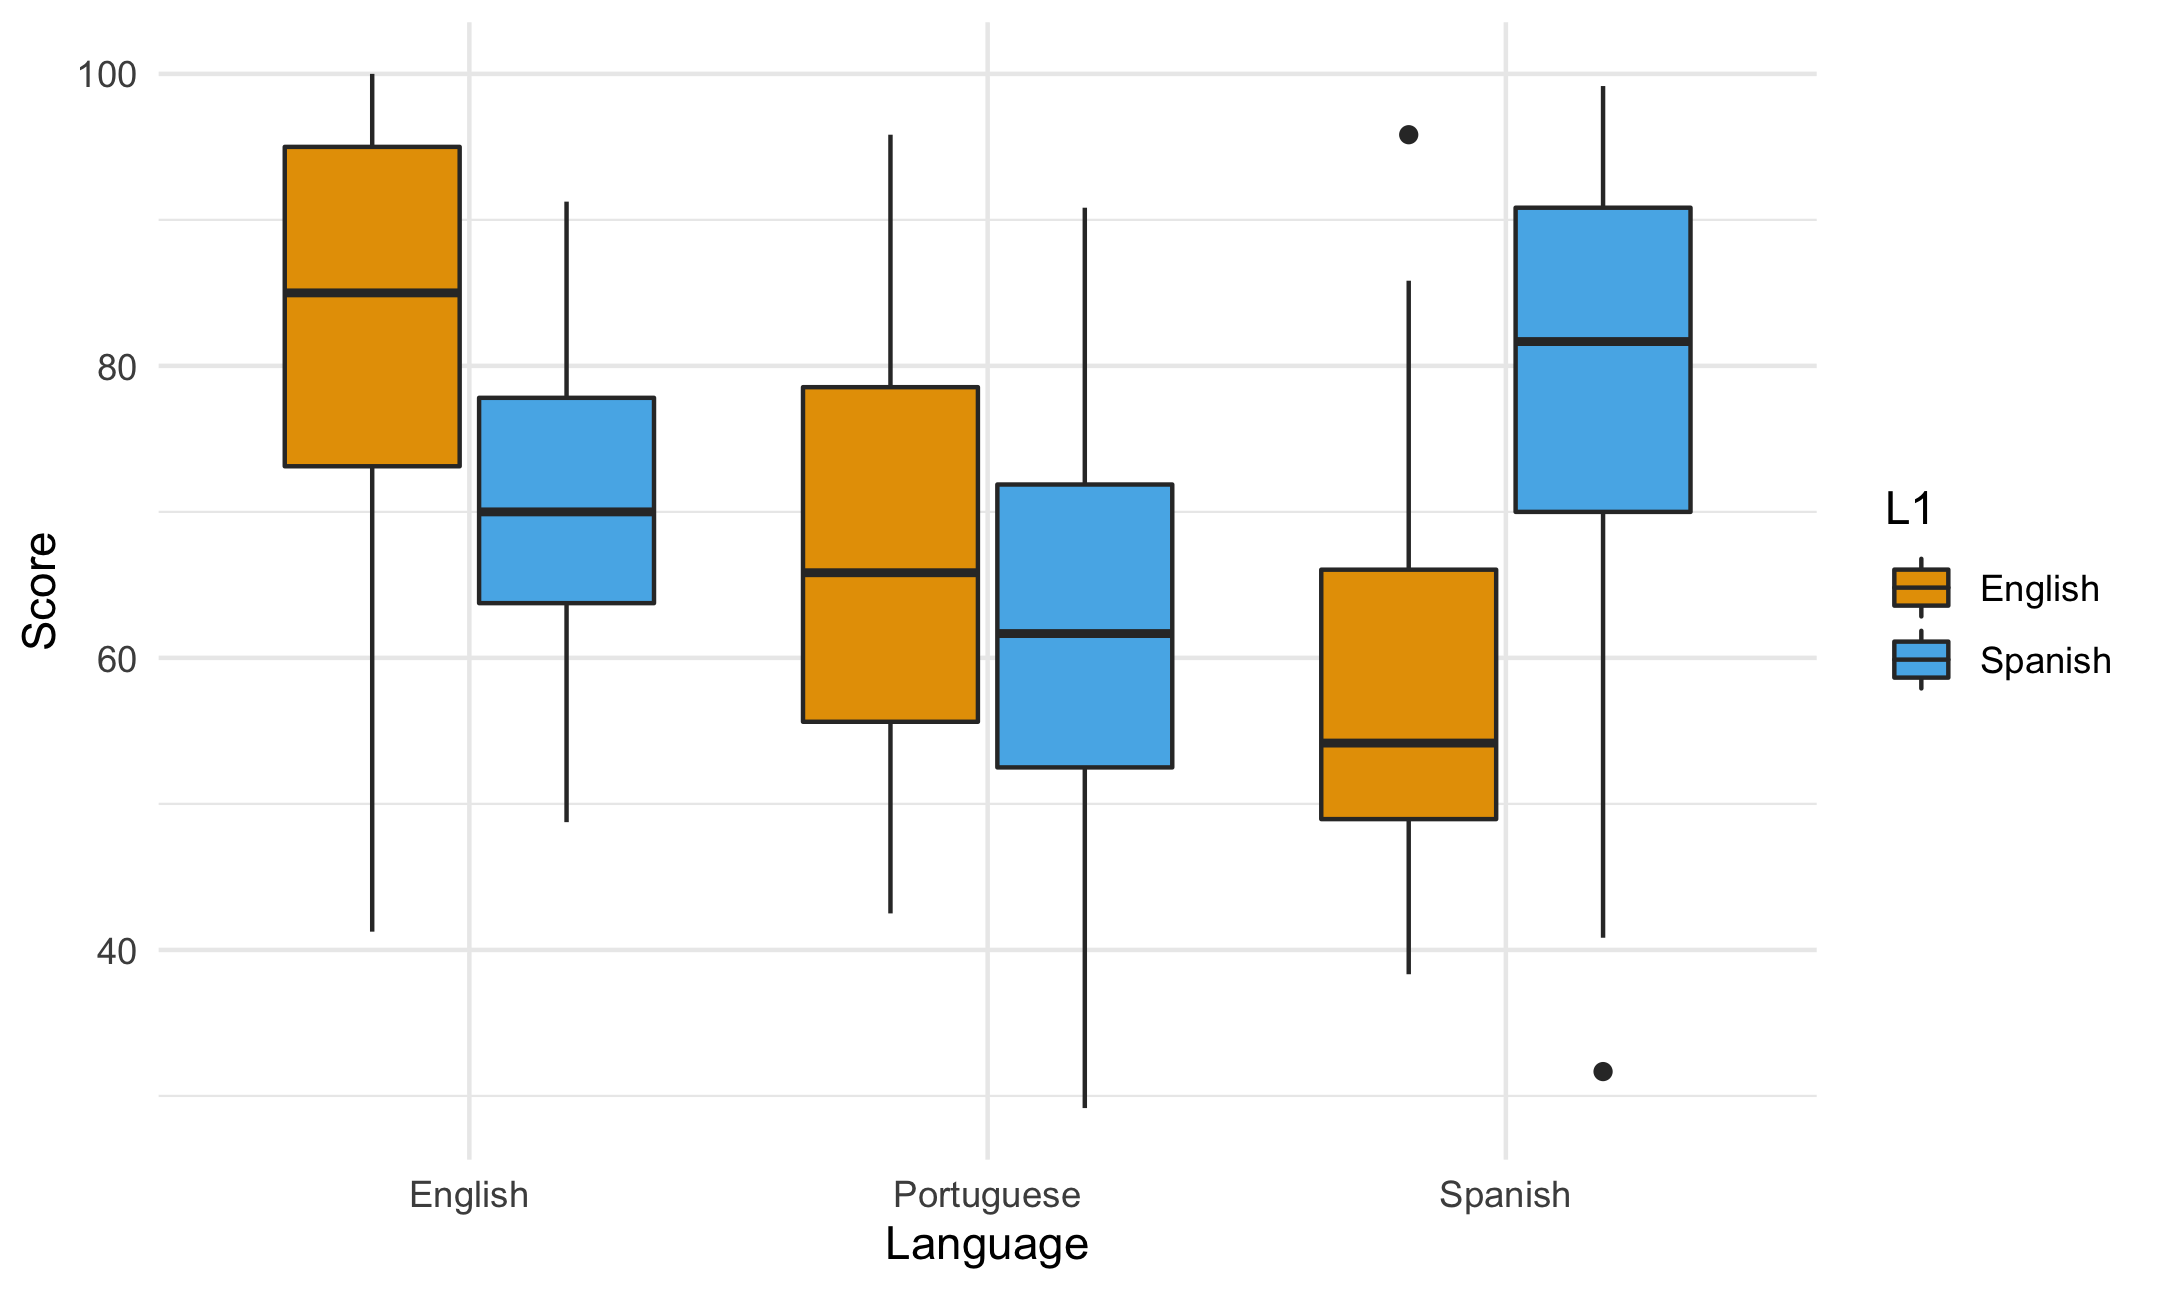
\includegraphics[width=425px]{figs/prof_plot} \caption{LexTALE score as a function of Language and Group.}\label{fig:prof-desc}
\end{figure}

\begin{longtable}[]{@{}rrrr@{}}
\caption{\label{tab:descproftable}A table of the proficiency scores by both groups in each language.}\tabularnewline
\toprule\noalign{}
L1 & Language & Mean Score & Range \\
\midrule\noalign{}
\endfirsthead
\toprule\noalign{}
L1 & Language & Mean Score & Range \\
\midrule\noalign{}
\endhead
\bottomrule\noalign{}
\endlastfoot
English & English & 82.64, sd = (14) & 41 - 100 \\
English & Portuguese & 65.57, sd = (13) & 42 - 96 \\
English & Spanish & 57.83, sd = (12) & 38 - 96 \\
Spanish & English & 70.47, sd = (11) & 39 - 91 \\
Spanish & Portuguese & 62.07, sd = (13) & 29 - 91 \\
Spanish & Spanish & 78.28, sd = (14) & 32 - 99 \\
\end{longtable}

\hypertarget{semantic-interpretation-task}{%
\subsubsection{Semantic Interpretation Task}\label{semantic-interpretation-task}}

The Semantic Interpretation task was designed to measure the perception of how adjective-noun order impacts determiner phrase (DP) interpretation.
In both Spanish and Portuguese, but not in English, whether an adjective is placed before a noun (\emph{el nuevo libro}) or after the noun (\emph{el libro nuevo}) can impact the meaning of the determiner phrase.
For example, \emph{el libro nuevo} refers to a book that has been newly acquired, but is not necessarily brand-new, where \emph{el neuvo libro} does refer to a brand new book.

This task was recreated on the basis of the description of the same task in the original study.
In both the original study and the present replication, during a trial, the participants saw one prompt at a time on the screen with two answer choices.
The participants submitted their choice by clicking either of the two answer choices with the mouse.
Like the original study, the task contained 10 experimental items which tested in each of a prenominal (n = 5) and postnominal conditions (n = 5).\\
A full list of the stimuli used, along with the correct answers, can be found in the supplementary materials.
Below is an example taken of the Semantic Interpretation task in Spanish taken directly from Rothman (2011).

\textbf{Prompt}

Mariela é uma velha amiga de Florence.

\emph{``Mariela is an old friend from Florence.''}

\textbf{Answer choices}

a.) \textbf{Muitos anos atrás eles são amigos.}

\emph{They have been friends for a long time.}

b.) Mariela é velha.

\emph{Mariela is old.}

\textbf{Prompt}

Naquela casa, mora um homem sozinho.

\emph{Only one man lives in that house.}

\textbf{Answer choices}

a.) O homem se sente sozinho.

\emph{The man feels lonely.}

b.) \textbf{Apenas um homem mora em casa.}

\emph{Just one man lives in the house.}

\hypertarget{context-based-collocation-task}{%
\subsubsection{Context-based Collocation Task}\label{context-based-collocation-task}}

A second task elicited production of adjectival DPs by way of context.
Again, like the original study, the participants in the present replication read a short story and had to fill in a blank at the end of the story with either a pre or post nominal adjective.
Like the Semantic Interpretation task, the participants saw one prompt at a time on the screen with two answer choices.
The participants submitted their choice by clicking either of the two answer choices with the mouse.
Like the original study, a total of 10 items were given to each participant, in which the correct answer of 5 items was a prenominal position and the remaining 5 were postnominal.
Below is an example adapted from the Context-based Collocation Task in Spanish taken directly from Rothman (2011).

\emph{Example}

Meus amigos não têm dinheiro. São \_\_\_\_\_\_\_\_\_\_\_\_\_\_\_ (pobres amigos/\textbf{amigos pobres}).

\emph{My friends do not have money. They are \_\_\_\_\_\_\_\_(unfortunate friends/poor friends)}

\hypertarget{procedure}{%
\subsection{Procedure}\label{procedure}}

Participants completed all tasks in a single experimental session in the in-browser platform Gorilla.sc (Anwyl-Irvine et al., 2018).
The session began with a brief history questionnaire, followed by the LexTALE proficiency tests (one in Spanish, English and Portuguese) and ended with the two experimental tasks.
Each participant completed the LexTALE in all three languages.
The order of the LexTALE test languages were randomized, so any combination of Spanish, English and Portuguese was possible.
The experiments paused briefly between tasks.
All data collection took place asynchronously online on the participant's computer.
All materials, scripts, and the document used to create this manuscript can be found on the Open Science Framework (\url{https://osf.io/t2vkp/}).

\hypertarget{statistical-analysis}{%
\subsection{Statistical analysis}\label{statistical-analysis}}

A replication of the analysis of the original study was carried out.
In the original study, two multilevel two-way ANOVAs for each of the tasks (the Semantic Interpretation and Context-based Collocation tasks) were done.
The assumptions of normal distribution of the residuals, homogeneity of the variance and sphericity were verified using the Performance package in R (Lüdecke et al., 2021).
In each model, the percentage of correct responses was analyzed as a function of item type (preposed or postposed), group (L1 Spanish, L1 English) and their interaction, with participant included as a random intercept.
Main effects and interactions were assessed using nested model comparisons and model assumptions were verified via visual inspections of Q-Q and residuals vs.~fitted plots.
Post-hoc tests of equivalence and t-tests were also run.
For the tests of equivalence, the equivalence bounds were Cohen's d = +/- .4.
The t-tests were run specifically so that they could be directly compared to the results of the test of equivalence and are run by default in the R function from the TOSTER package (Caldwell, 2022).
In all cases, alpha was set to .05.
Data was prepared for the analyses using a series of scripts in R using the tidyverse package (Wickham et al., 2019).
The final dataframe submitted for the analysis contained the four total columns: a participant identification number, their L1, condition (pre or post nominal) and that individual's total number correct (out of 5 possible).
The proficiency tests were scored and standardized using a separate scripts.
These scripts are openly available on the Open Science Framework.

\hypertarget{results}{%
\section{Results}\label{results}}

Figure \ref{fig:sem-desc} shows the average correct responses (out of 5) for the Semantic Interpretation task by both groups, while figure \ref{fig:cmc-desc} shows the same information for the Context-based collocation task by both groups.
The means and standard deviations for each case are present just above each bar.
Overall, the participants were more often correct in the postposed condition in both tasks.

\begin{figure}
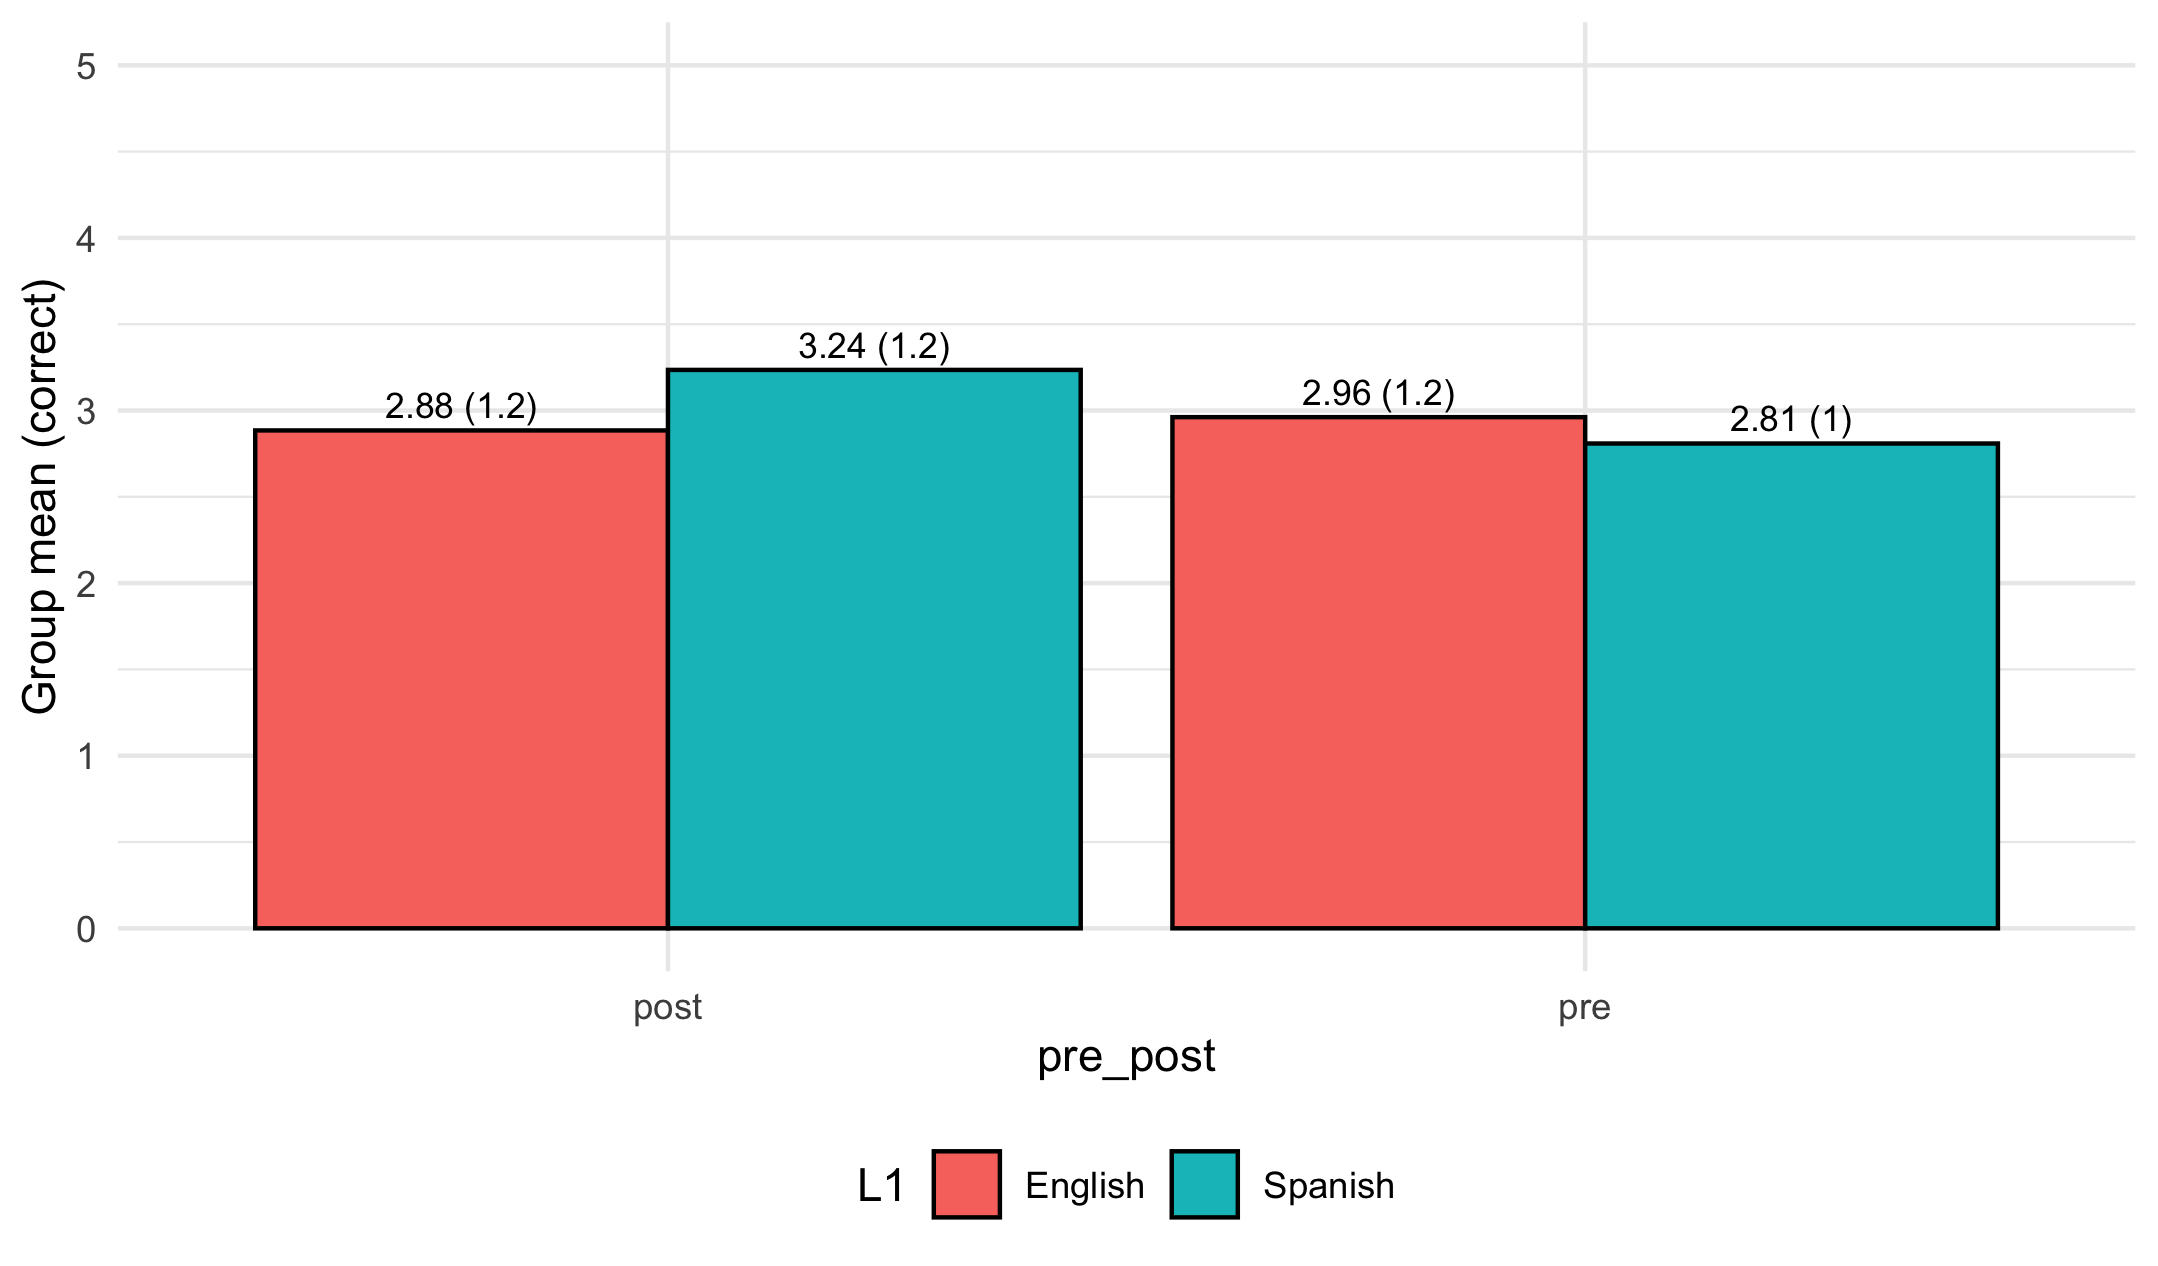
\includegraphics[width=425px]{figs/semantic_desc} \caption{Average Number of correct answers in the Semantic Interpretation Task.}\label{fig:sem-desc}
\end{figure}

\begin{figure}
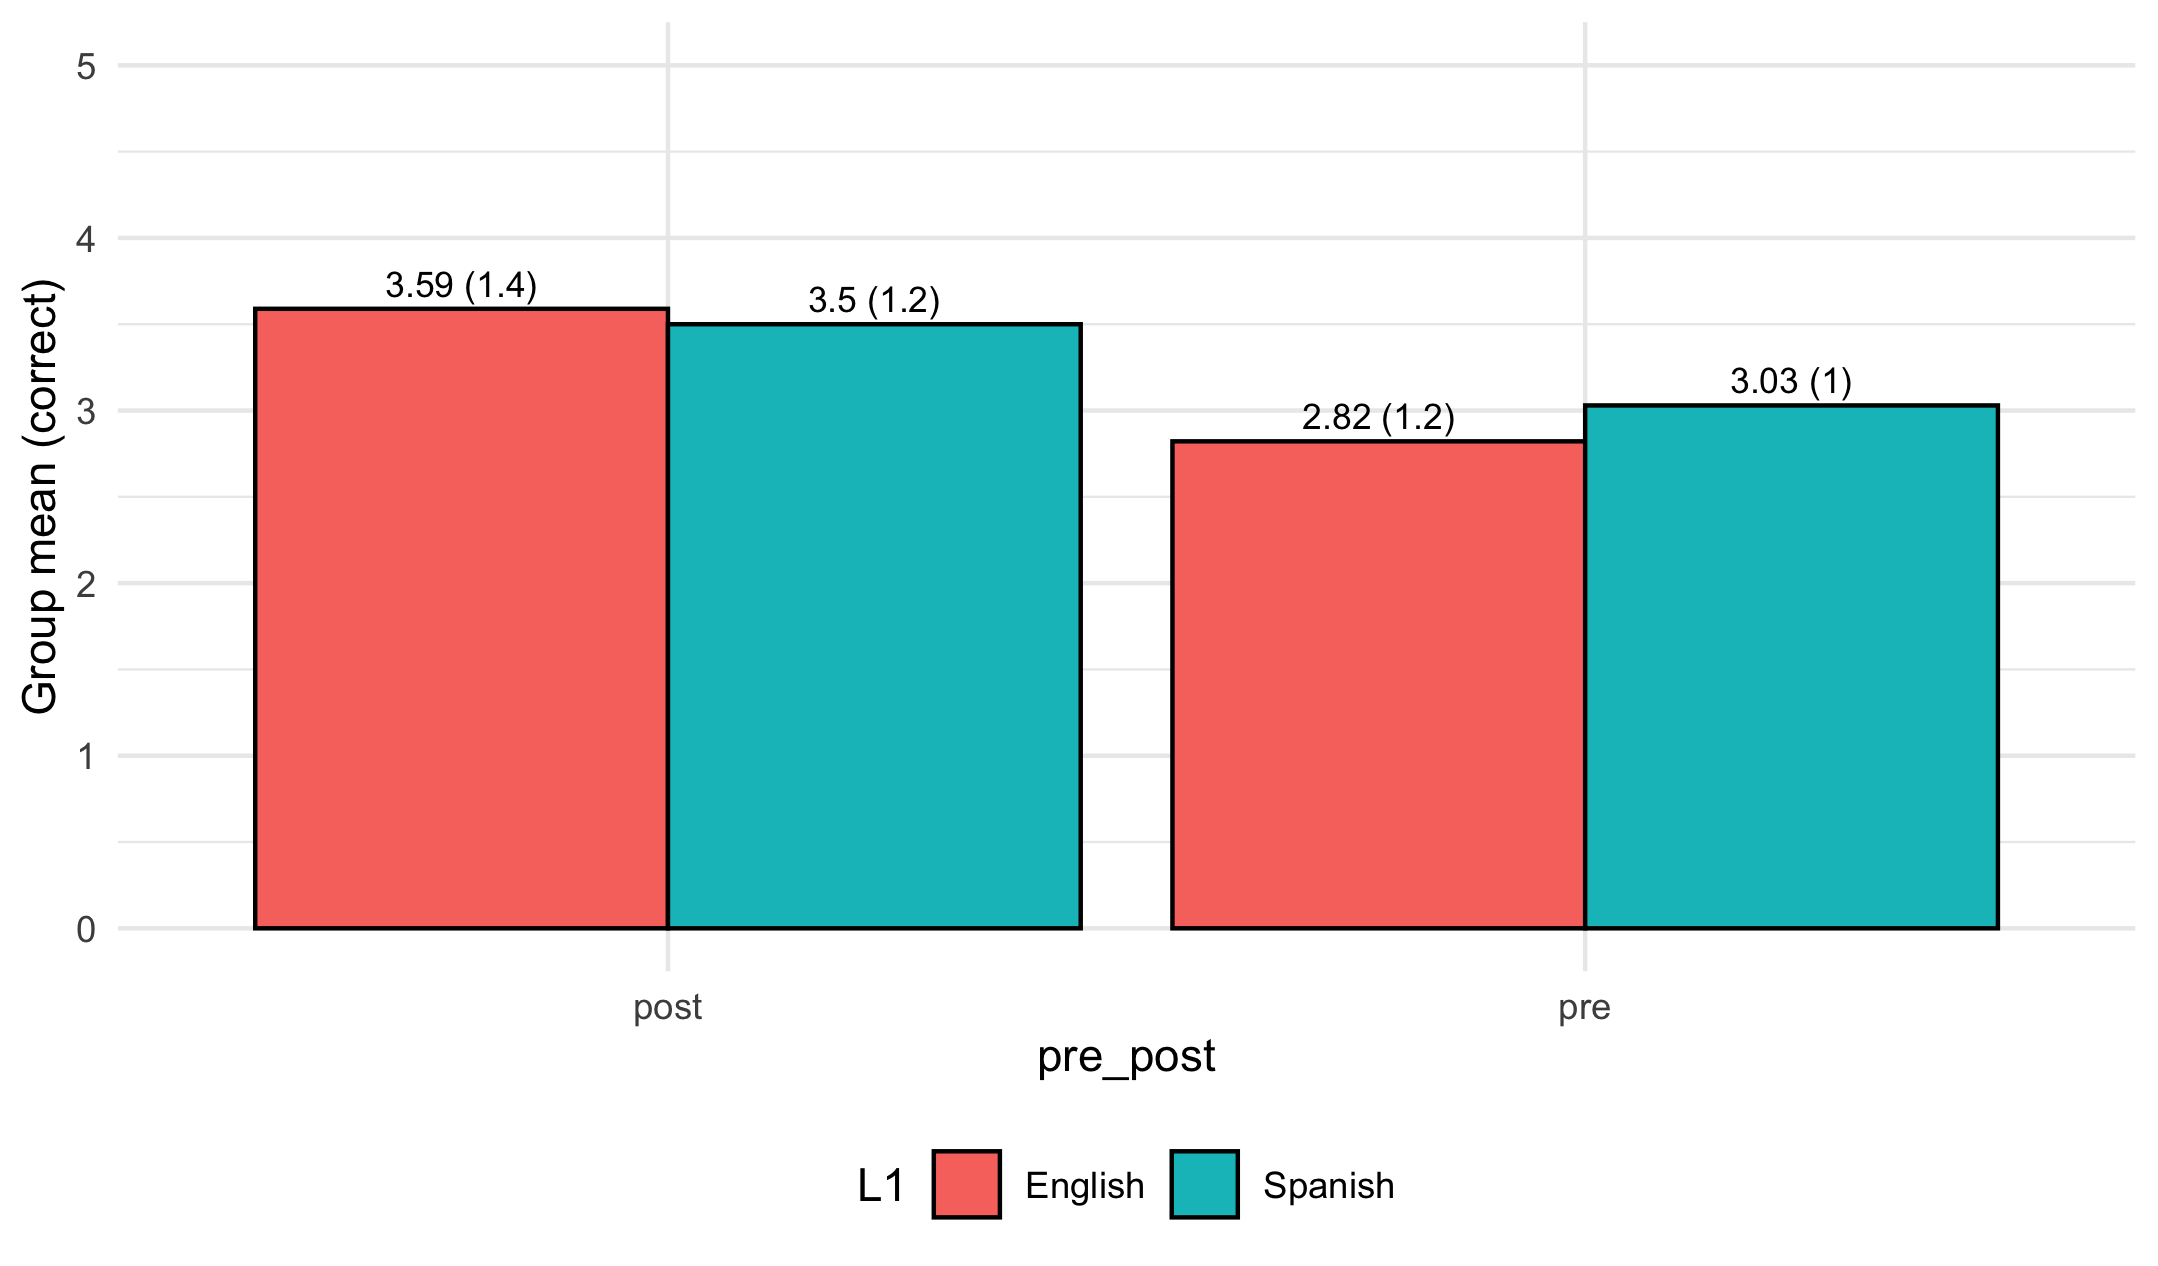
\includegraphics[width=425px]{figs/cbc_desc} \caption{Average Number of correct answers in the Context-based Collocation Task.}\label{fig:cmc-desc}
\end{figure}

\hypertarget{replication-of-the-original-analysis}{%
\subsubsection{Replication of the original analysis}\label{replication-of-the-original-analysis}}

There was no main effect for group in the ANOVA for the collocation task, F(1, 213) = 0.47, p = 0.50 or the group by position interaction (F(1, 213) = 1.37, p \textless{} .05).
There was, however, a main effect for position (pre vs.~post), F(1, 213) = 36.06, p \textless{} .05.
In the interpretation task, there was also no main effect for group, F(1, 209) = 0.22, p = 0.64.
Like the collocation task, there was a main effect for position (pre vs.~post), F(1, 209) = 8.41, p \textless{} .05.
There was also a group by position interaction, F(1, 209) = 6.72, p \textless{} .05.

\hypertarget{test-of-equivalence}{%
\subsubsection{Test of Equivalence}\label{test-of-equivalence}}

In addition to each test of equivalence, a Welch's Two Sample t-test was carried out to determine whether, while also potentially being practically equivalent, a comparison would also be statistically different (see e.g. Lakens et al., 2018).
Each test was run between groups (L1 English and L1 Spanish) for either preposed or postposed adjectives in both the semantic interpretation task and collocation task.

\hypertarget{postposed-collocation-task}{%
\subsection{Postposed collocation task}\label{postposed-collocation-task}}

The equivalence test was significant in the postposed collocation task, t(207) = -2.65, p \textless{} .05.
The equivalence bounds were d = +/- .4 or +/- 0.51 in raw units (answers correct).
The observed effect was a mean difference of 0.05 (90\% CI -0.24 - 0.34) in standardized units or 0.04 (90\% CI -0.19 - 0.26) in raw units.
The t-test was not significant, t(207) = 0.28, p = 0.78.
Given these results, we can conclude that the groups were not different from 0 and statistically practically equivalent in their number of correct answers in the postposed condition in the collocation task.

\hypertarget{preposed-collocation-task}{%
\subsection{Preposed collocation task}\label{preposed-collocation-task}}

In the preposed condition on the collocation task, the test of equivalence was significant for the upper bound \(\Delta\)U, t(194.23) = -4.28, p \textless{} .05, but not at the lower bound, \(\Delta\)L, t(194.23) = 1.54, p = 0.06.
The equivalence bounds were d = +/- .4 or +/- 0.45 in raw units (answers correct).
The observed effect was a mean difference of -0.21 (90\% CI -0.47 - 0.04) in standardized units or -0.19 (90\% CI -0.41 - 0.04) in raw units.
The t-test was also not significant, t(194) = -1.37, p = 0.17.
Taken together, these results suggest that the effect is not different from zero and also not practically equivalent within a small effect size.
In other words, in this case, there was insufficient evidence to come to a conclusion.

\hypertarget{postposed-semantic-interpretation-task}{%
\subsection{Postposed Semantic interpretation task}\label{postposed-semantic-interpretation-task}}

The equivalence test was significant in the postposed semantic interpretation task, t(199) = -4.12, p \textless{} 0.05.
The equivalence bounds were d = +/- .4 or +/- 0.48 in raw units (answers correct).
The observed effect was a mean difference of -0.20 (90\% CI -0.48 - 0.07) in standardized units or -0.17 (90\% CI -0.40 - 0.06) in raw units.
The t-test was not significant, t(198.98) = 0.28, p = 0.78.
Given these results, we can conclude that the groups were not different from 0 and statistically practically equivalent in their number of correct answers in the postposed condition in the collocation task.

\hypertarget{preposed-semantic-interpretation-task}{%
\subsection{Preposed Semantic interpretation task}\label{preposed-semantic-interpretation-task}}

In the preposed condition on the semantic interpretation task, the test of equivalence was not significant for the upper bound \(\Delta\)U, t(194.23) = -4.28, p \textless{} .05, nor was it at the lower bound, \(\Delta\)L, t(194.23) = 1.54, p = 0.06.
The equivalence bounds were d = +/- .4 or +/- 0.45 in raw units (answers correct).
The observed effect was a mean difference of -0.21 (90\% CI -0.47 - 0.04) in standardized units or -0.19 (90\% CI -0.41 - 0.04) in raw units.
The t-test was significant, t(198.71) = 2.10, p = 0.04.
Taken together, these results suggest that the groups were statistically different in their number of correct answers and not practically equivalent within a small effect size.

\hypertarget{discussion-and-conclusion}{%
\section{Discussion and conclusion}\label{discussion-and-conclusion}}

\begin{longtable}[]{@{}lrr@{}}
\caption{\label{tab:summaryanovas}Summary of the Analyses of Variance in both tasks}\tabularnewline
\toprule\noalign{}
\endfirsthead
\endhead
\bottomrule\noalign{}
\endlastfoot
Task & Collocation Task & Semantic Interpretation Task \\
Group & no & no \\
ANOVA\_position & yes & yes \\
ANOVA\_interaction & no & yes \\
Replication & Partial & Partial \\
\end{longtable}

Table \ref{tab:summaryanovas} summarizes the results of the replication of the original analyses.
Overall, the results of the two ANOVAs point to a partial replication of the original analysis.
A full replication for the purpose of the present study would have included no main effect of group (which was replicated for both tasks) and no group x position interaction (which was only replicated for one task).
Additionally, unlike the original study, the replication did find main effects for position in both tasks.
While the non-null results were not expected, these differences are not discussed in great detail here due to space limitations.

The primary purpose of the present replication was to investigate whether the lack of main effect of group was also practically equivalent at a higher sample size.
The results indicate that this was the case only some of the time.
Table \ref{tab:summaryttests} details results of the tests of equivalence.
The four total tests compared the number of correct answers out of five for both tasks in preposed and postposed positions.
The results showed that two of the four comparisons were practically equivalent, while they other two were not, when the equivalence bounds were d = +/- .4.

\begin{longtable}[]{@{}rrrr@{}}
\caption{\label{tab:summaryttests}Summary of the results from the tests of equivalence and t-tests}\tabularnewline
\toprule\noalign{}
Position & Task & TOST & t\_test \\
\midrule\noalign{}
\endfirsthead
\toprule\noalign{}
Position & Task & TOST & t\_test \\
\midrule\noalign{}
\endhead
\bottomrule\noalign{}
\endlastfoot
pre & Collocation Task & no & no \\
post & Collocation Task & yes & no \\
pre & Semantic Interpretation Task & no & yes \\
post & Semantic Interpretation Task & yes & no \\
\end{longtable}

These results showed that null effects do not always entail practical equivalence, and suggest that statistical methods of determining practical equivalence, such as equivalence testing, can be useful in L2 and L3 studies moving forward.
Equivalence testing arguably allows for the marriage of our statistical tools and theory, since the equivalence bounds are ideally be determined on the basis of the smallest important difference in practice.
In the present study, d = +/- .4 was considered as the SESOI based on a recent meta-analysis of effect sizes in L2 research (Plonsky \& Oswald, 2014).
This number came from the approximately 25th percentile of the total effects and was considered small, whereas the 50th percentile was considered a medium effect (d = +/- .7) and 75th percentile was considered large (d = +/- 1).
These more specific guidelines stand in contrast to the recommendations of Cohen (2013), who proposed initial bench marks of .2, .5, and .8, as small, medium, and large effect sizes.
While researchers in L2 or L3 research could use the new benchmarks proposed by Plonsky and Oswald (2014) as a general guideline, more fine-grained approaches have also been proposed such as anchor-based methods or the subjective experience of participant perception in order to justify the smallest effect size of interest (SESOI) (see Anvari \& Lakens, 2021).

Once one has determined the SESOI, then it can be determined how many participants are necessary in each group by running a power analysis, regardless of whether one's aim is to demonstrate that groups or conditions are distinct or equivalent.
Figure \ref{fig:pc} shows the needed participants per group to detect practical equivalence at a power level of .8 (alpha = .05) according do the smallest effect size of interest ranging from d = +/-.1 to +/- 1.
The smallest effect size of interest was used as the equivalence bounds, meaning that any effect less than the SESOI was considered practically equivalent.
It is clear from the figure that evidence for the null hypothesis requires a rather large sample in the event that a very small effect is considered meaningful.
For example, if the SESOI is d = +/- .1, then 1713 participants are needed per group to achieve a power level of .8.
On the other hand, if only a large effect is considered meaningful, such as d = +/- 1, then only 17 participants are needed per group.
Figure \ref{fig:pct} shows the how many participants are needed to detect any difference when the true effect size is the number on the x-axis at a power level of .8.
In other words, a particular SESOI and number of participants per group results in a probability of .8 of detecting any significant difference, and a probability of .2 that the results will falsely be negative.
In each of the ten cases effect sizes, slightly more participants are needed per group to detect practical equivalence.
For example, d = +/- .4 needs 98 per group to be able to detect a difference at a power level of .8, but 107 per group to determine practical equivalence.

\begin{figure}
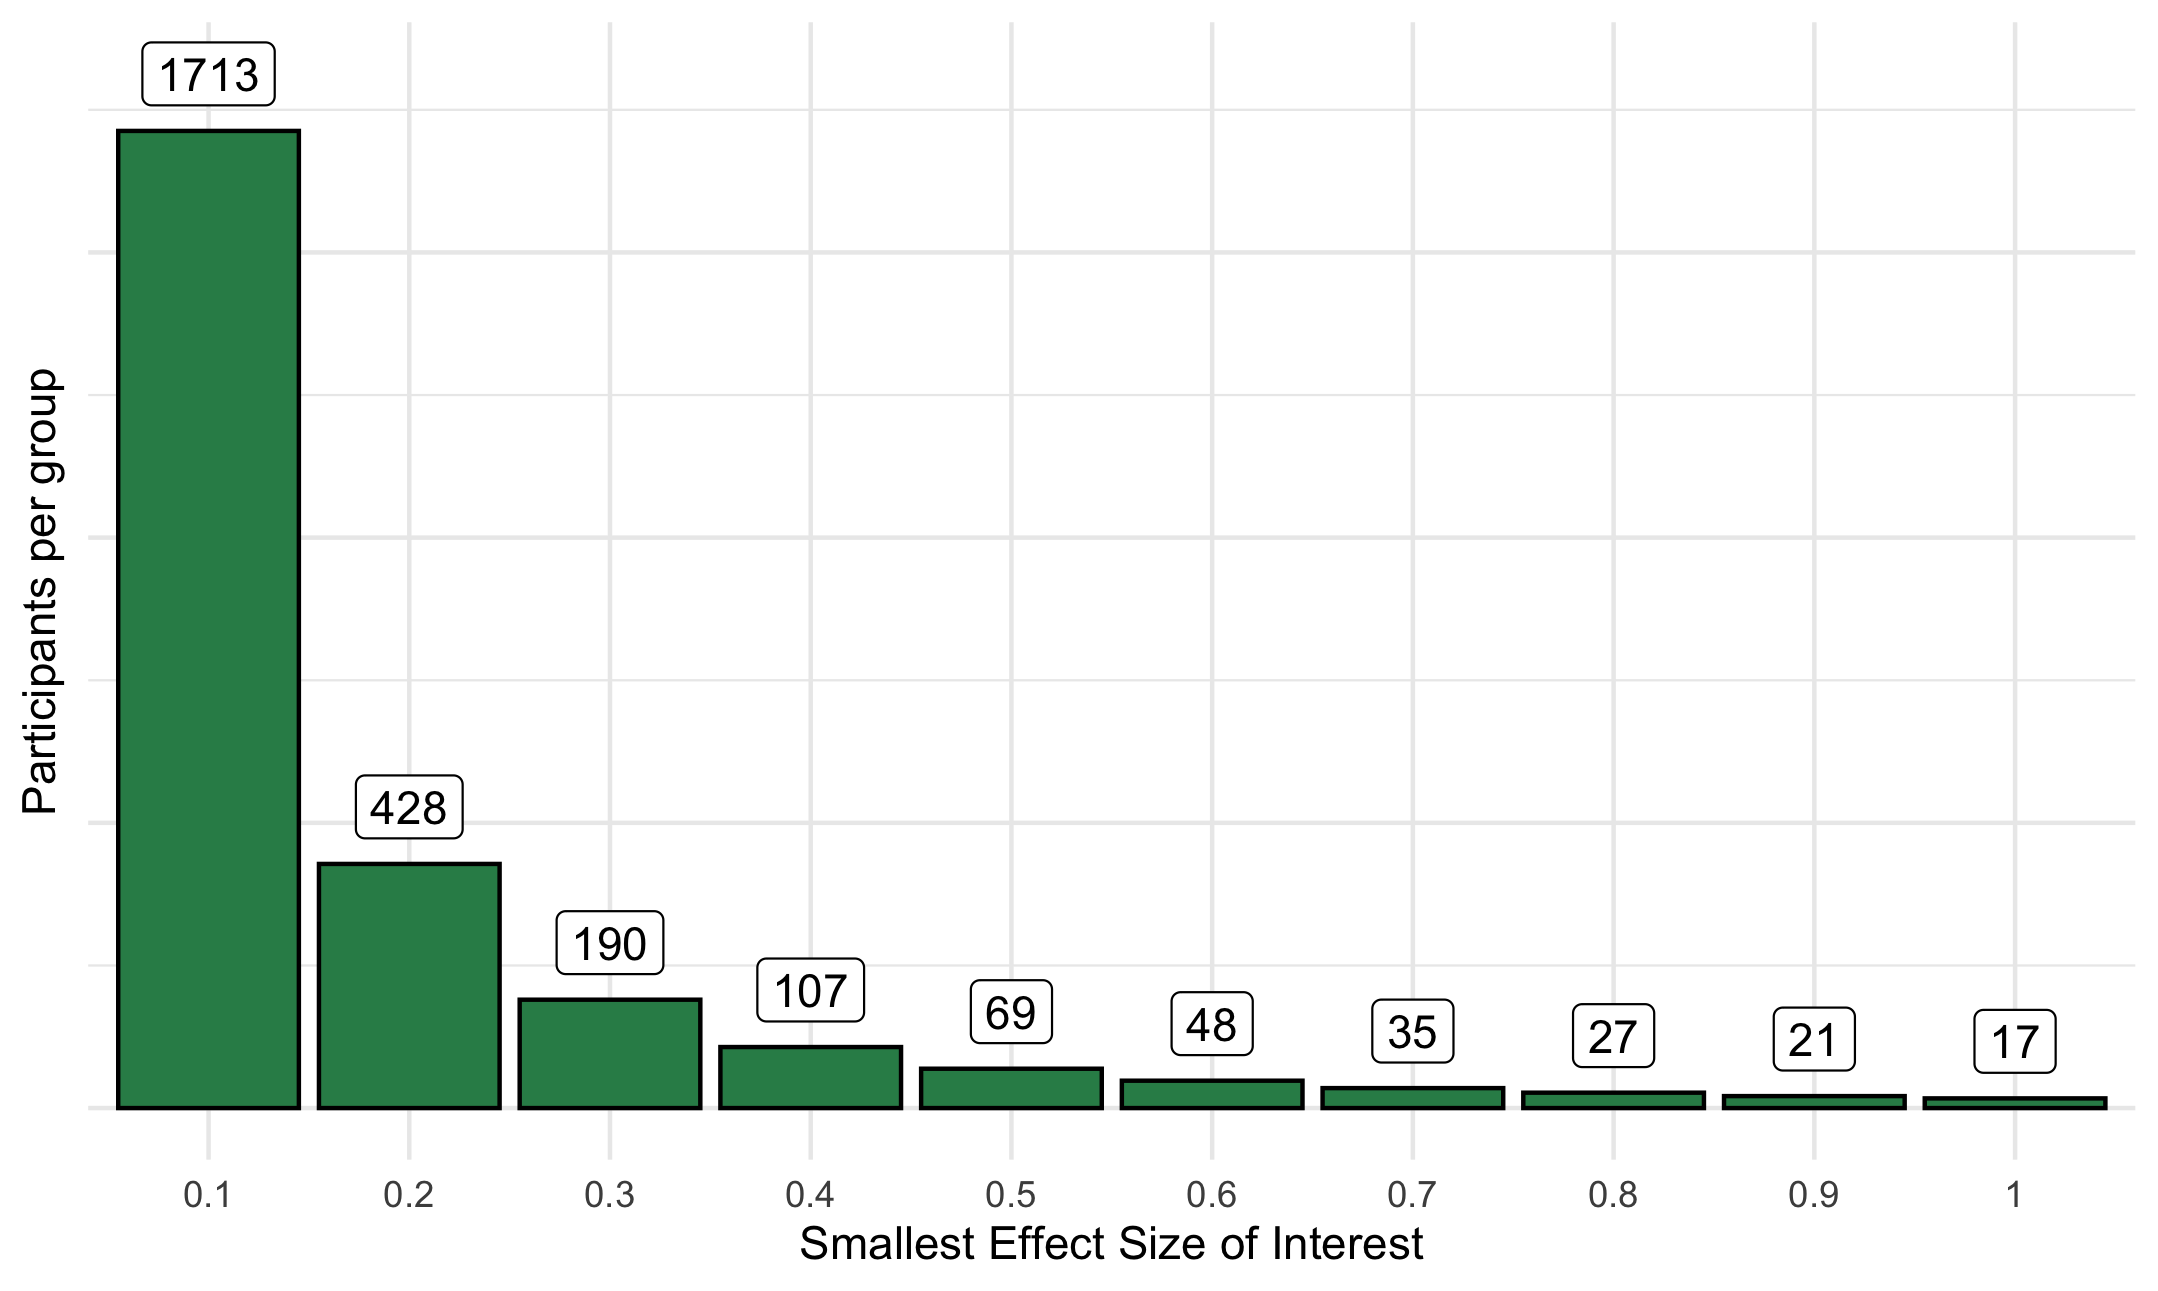
\includegraphics[width=425px]{figs/pc} \caption{Number of participants needed per effect size to detect practical equivalence.}\label{fig:pc}
\end{figure}

\begin{figure}
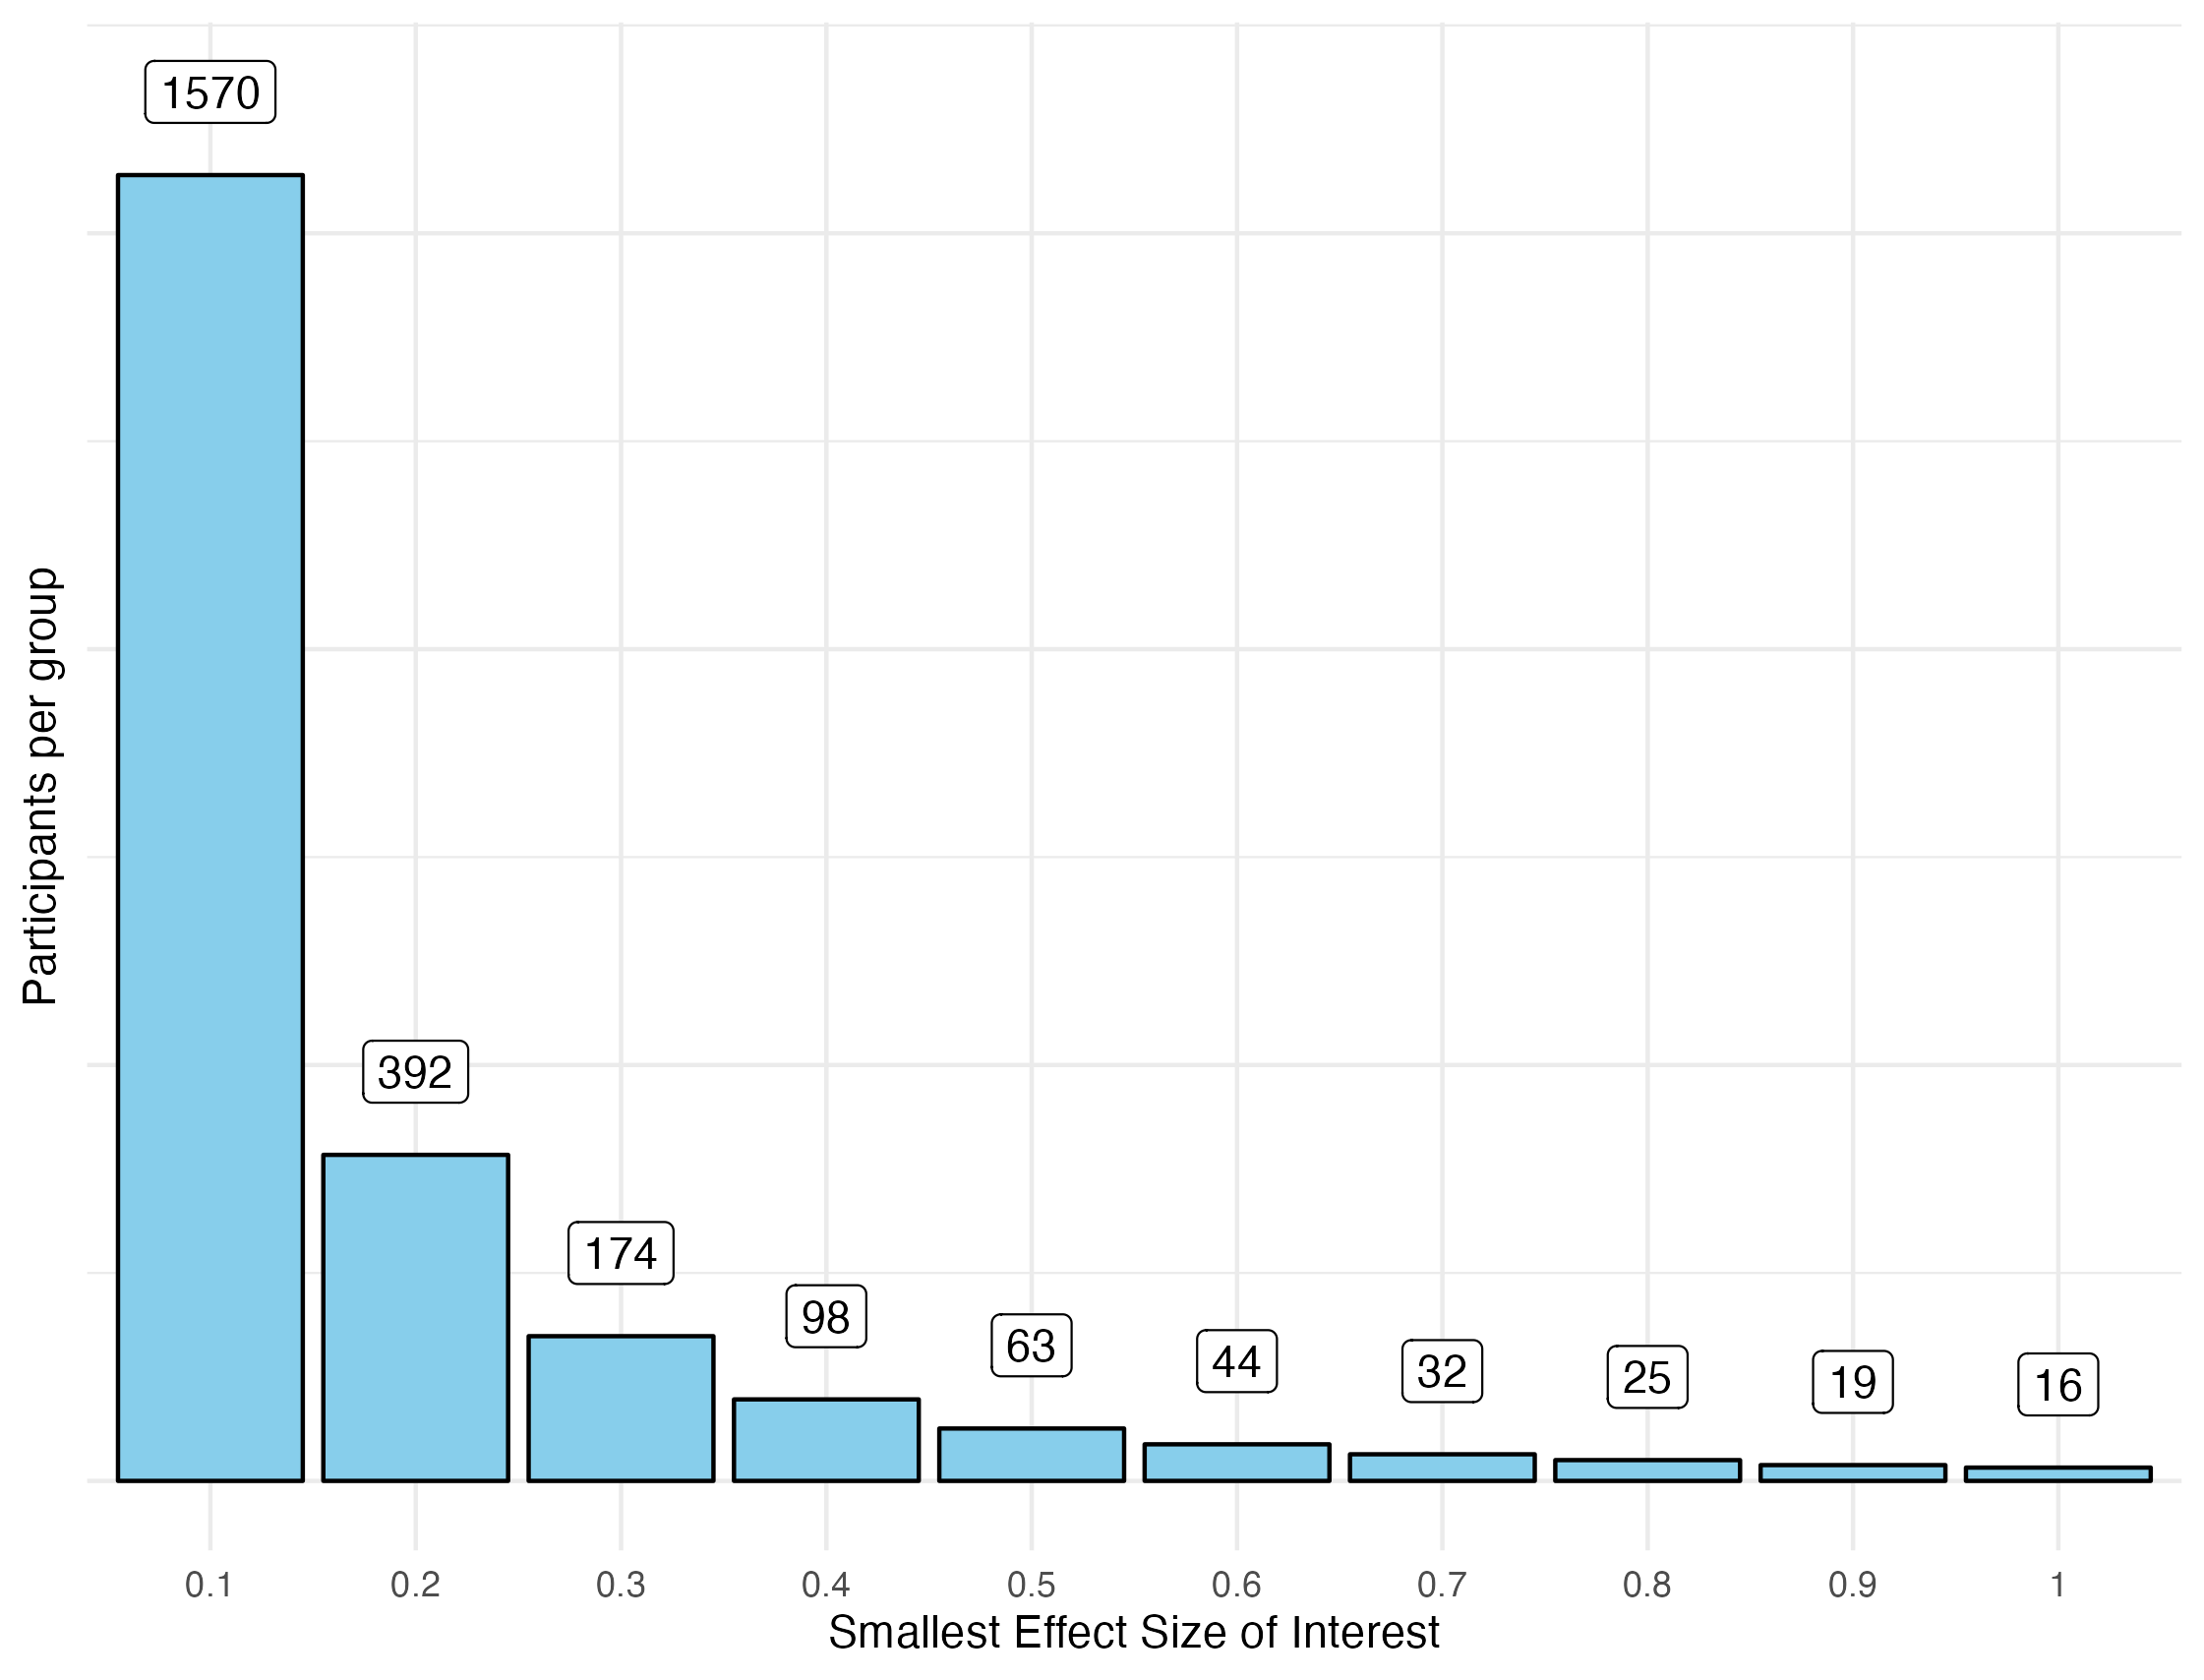
\includegraphics[width=425px]{figs/pc_t} \caption{Number of participants needed per effect size to detect any significant difference.}\label{fig:pct}
\end{figure}

Although the present work largely advocates for larger samples and the use of equivalence testing, this may not be practical to every study.
It is important to note that, especially in studies of multilinguals, it can be very difficult to find statistically powered samples of participants that can be justifiably added to a single group.
This occurs, in part, due to the wide variety of variability in bilingual populations.
Despite these potential issues, a lack of power is not necessarily a reason not to carry out a study.
Rather, it is reason to temper the conclusions from a given experiment, or to increase the observations drawn from an individual participant.
For instance, in the case of the original study, a power analysis reveals that the probability (assuming a similar standard deviation to the on collected here) of a significant equivalence test (power = .8, alpha = .05, d = +/- .4) was essentially 0.
As a result, a more appropriate conclusion based on the results of the statistical tests in the original study would been that the result was not significantly different nor was there sufficient evidence that it was the same.
In other words, the results of the original study were inconclusive.

It is important to note, also, that (as pointed out by an anonymous reviewer), the frequentist approach to statistical analysis in concerned with the long run outcome of an experiment theoretically being repeated a number of times.
In this view, if a study with a true underlying effect is hypothetically repeated 100 times, then 5 of these will be false positives (or the level of the significance threshold), and 20 will be false negatives (if the power level is .8).
As a result, the result of a single study is in itself inconclusive since there is no way to verify whether it is one of the false positive or false negative results on the basis of its own existence, but rather it would need to be evaluated in conjunction with later repetitions.

As a result, the higher probability that many low sample studies will produce false negative findings, they can and should still be published, since they can be analyzed in aggregate.
The lack of tolerance for inconclusive, or null results, has been described as the file drawer problem (Rosenthal, 1979).
In the worst-case scenario form of this view, the bias to publish only significant result could theoretically result in only false-positive studies being published.
That is, using a significance threshold of .05, 5 out of 100 independent studies showing a significant difference are published while 95 null findings are put in the ``file drawer'' and not published.
Tools exist such at meta-analysis allow for the cumulative evaluation of the findings, whether or not they are underpowered or significant.
By using meta-analysis, once underpowered samples reduce the risk of false negative findings (type II error).
This, taken together with the publication of null or inconclusive findings, the probability of false positive findings (type I error) can also be reduced.

It should also be noted that the Test of Equivalence utilized by the present study is simply
one option for determining practical equivalence, and that other approaches may be more appropriate for distinct experimental designs.
For example, Bayesian methods can establish a Region of Practical Equivalence (ROPE) and compare it to the Highest Density Interval (HDI) in order to provide evidence of equivalence (Kruschke, 2018).
More recently, the use of the Bayes Factor has also been proposed (Linde et al., 2023).

One important aspect in equivalence testing is to determine what differences are meaningful, and thus, where to set the equivalence bounds.
In their current forms, none of the L3 models specify exactly how much difference between groups on a given task constitutes evidence of transfer.
Recall that the present study used a general benchmark of d = +/- .4 as the equivalence bounds based on the meta-analysis of Plonsky and Oswald (2014).
Interestingly, if the bounds had been set to d = +/- .5, all four of the tests of equivalence would have been significant.
To put this in terms of correct answers out of 5, given a pooled standard deviation of 1.2, the mean difference between groups would be .6 answers correct (group A has 3 answers correct and group B has 3.6 and we would say they are practically equivalent) as opposed to the chosen equivalence bounds of d = +/- .4 or .48 (such as 3 answers correct vs.~3.48 answers correct).
As it stands, neither of these equivalence bounds are justified by more than being a general guideline.
Both the Linguistic Proximity Model (Westergaard et al., 2017, 2022) and the Typological Primacy Model (Rothman, 2011, 2015) explain the finding that both groups have access to Spanish in their Brazilian Portuguese, and that order of acquisition effects do not seem to impact determiner phrases perception and production in this particular language combination.
One important prediction which differentiates these models is the idea that, according to the LPM, L3 users can be influenced by both known languages simultaneously.
It is argued that this influence can be seen by intermediate performance in a subtractive design.
That is, in this situation an L3 speaker, such as an L1 English-L2 Spanish-L3 Brazilian Portuguese speaker would be compared to two groups of L2 Brazilian Portuguese speakers (with L1 English and L1 Spanish).
Depending on the linguistic structure, the L3 group is predicted here to perform more poorly than one group, but better than another.
The implications of the present work suggest that it is necessary to determine what specific difference entails intermediate performance and when a difference is so small, even if it is statistically significant, that it is negligible

Finally, an unexpected finding is that in the pre-posed interpretation task, the L1 Spanish group exhibits a significantly lower proportion of correct responses than the L1 English group.
An anonymous reviewer suggested that it is possible that the Cumulative Threshold Input Hypothesis (Cabrelli \& Iverson, 2023) might be able to explain this finding, given that participants are not at the initial stages of learning Portuguese.
However, the Cumulative Threshold Input Hypothesis suggests that, in L3 development, learners overcome non-facilitative transfer faster when they have a lower amount of total input in the source language.
In this case, the pre-posed condition is a (more) English-like production, where post-posed is always Spanish-like.
As a result, Cumulative Threshold Input Hypothesis would predict that the correctness in the pre-posed condition should be negatively correlated to the amount of input in English, so the Spanish group should display higher accuracy than the English group.
However, this difference does not hold in the Context-based collocation task, and it is rather small (a difference of .15 answers correct, d = .13).
Given the size of this effect, lack of a similar effect or trend in the collocation task and the sample involved, it is not immediately clear whether this difference can be explained by theory or simply random error.

Future replication research in the field of L3 acquisition should, when possible, aim to reasonably increase the samples of participants or observations in order to re-examine whether previous statistical findings warrant narrative theoretical conclusions. In particular, future work could replicate seminal findings in the Linguistic Proximity Model (Westergaard et al., 2017), which used intermediate performance of an L3 group relative to two L2 groups as evidence for simultaneous L1 and L2 influence on the L3. That is, the model only predicts the direction of effects based on linguistic representations but not the specific magnitude of these effects. In other words, a replication could provide insight into how big of a difference begins to constitute intermediate performance and at which point a difference is so small that it is not meaningful or is not statistically powered enough to be detected. Ultimately, in L3 acquisition and behavioral research in general, future work should aim to uncover not just the direction of an expected effect, but also its size.

In conclusion, the present work was a approximate replication of Rothman (2011). The study recreated a Semantic Interpretation task and Context-based Collocation task for L3 speakers of Brazilian Portuguese (who spoke L1 English and L2 Spanish or L1 Spanish and L2 English).
In the original study, no main effect or interactions were found, suggesting that both groups were influenced by Spanish in their L3. Out of 4 possible null main effects and interaction in the replication, only 2 replicated (were null), and 2 were statistically significant. As a novelty, the present replication also used Tests of Equivalence to determine whether these null effects in tests designed to detect differences would also be significant in a test designed to provide evidence of practical equivalence. These results showed than none of the four Tests of Equivalence were significant.
The present work suggests that, overall, for experiments in which statistical equivalence or differences are being used to argue for theory, both of these outcomes should have clearly specified criteria for their evaluation.

\newpage

\hypertarget{references}{%
\section{References}\label{references}}

\begingroup
\setlength{\parindent}{-0.5in}
\setlength{\leftskip}{0.5in}

\hypertarget{refs}{}
\begin{CSLReferences}{1}{0}
\leavevmode\vadjust pre{\hypertarget{ref-altman1995statistics}{}}%
Altman, D. G., \& Bland, J. M. (1995). Statistics notes: Absence of evidence is not evidence of absence. \emph{Bmj}, \emph{311}(7003), 485.

\leavevmode\vadjust pre{\hypertarget{ref-anvari2021using}{}}%
Anvari, F., \& Lakens, D. (2021). Using anchor-based methods to determine the smallest effect size of interest. \emph{Journal of Experimental Social Psychology}, \emph{96}, 104159.

\leavevmode\vadjust pre{\hypertarget{ref-anwyl2018gorillas}{}}%
Anwyl-Irvine, A., Massonnié, J., Flitton, A., Kirkham, N., \& Evershed, J. (2018). Gorillas in our midst: Gorilla. sc. \emph{Behavior Research Methods}.

\leavevmode\vadjust pre{\hypertarget{ref-bardel2007role}{}}%
Bardel, C., \& Falk, Y. (2007). The role of the second language in third language acquisition: The case of germanic syntax. \emph{Second Language Research}, \emph{23}(4), 459--484.

\leavevmode\vadjust pre{\hypertarget{ref-bardel2012l2}{}}%
Bardel, C., \& Falk, Y. (2012). The L2 status factor and the declarative/procedural distinction. \emph{Third Language Acquisition in Adulthood}, \emph{46}, 61--78.

\leavevmode\vadjust pre{\hypertarget{ref-borg2013acquisition}{}}%
Borg, K. (2013). The acquisition of future of probability in L3 spanish. \emph{Proceedings of the 12th Generative Approaches to Second Language Acquisition Conference}, 11--21.

\leavevmode\vadjust pre{\hypertarget{ref-cabrelli2023learners}{}}%
Cabrelli, J., \& Iverson, M. (2023). Why do learners overcome non-facilitative transfer faster from an L2 than an L1? The cumulative input threshold hypothesis. \emph{International Journal of Multilingualism}, 1--27.

\leavevmode\vadjust pre{\hypertarget{ref-caldwell2022exploring}{}}%
Caldwell, A. R. (2022). \emph{Exploring equivalence testing with the updated TOSTER r package}.

\leavevmode\vadjust pre{\hypertarget{ref-cohen2013statistical}{}}%
Cohen, J. (2013). \emph{Statistical power analysis for the behavioral sciences}. Academic press.

\leavevmode\vadjust pre{\hypertarget{ref-falk2017pronouns}{}}%
Falk, Y. (2017). On pronouns that drop (out of german). \emph{L3 Syntactic Transfer: Models, New Developments and Implications}, 127--142.

\leavevmode\vadjust pre{\hypertarget{ref-falk2011object}{}}%
Falk, Y., \& Bardel, C. (2011). Object pronouns in german L3 syntax: Evidence for the L2 status factor. \emph{Second Language Research}, \emph{27}(1), 59--82.

\leavevmode\vadjust pre{\hypertarget{ref-foote2009transfer}{}}%
Foote, R. (2009). Transfer in L3 acquisition: The role of typology. \emph{Third Language Acquisition and Universal Grammar}, \emph{37}, 89.

\leavevmode\vadjust pre{\hypertarget{ref-hermas2010language}{}}%
Hermas, A. (2010). Language acquisition as computational resetting: Verb movement in L3 initial state. \emph{International Journal of Multilingualism}, \emph{7}(4), 343--362.

\leavevmode\vadjust pre{\hypertarget{ref-hermas2014multilingual}{}}%
Hermas, A. (2014). Multilingual transfer: L1 morphosyntax in L3 english. \emph{International Journal of Language Studies}, \emph{8}(2), 1--24.

\leavevmode\vadjust pre{\hypertarget{ref-hopp2019cross}{}}%
Hopp, H. (2019). Cross-linguistic influence in the child third language acquisition of grammar: Sentence comprehension and production among turkish-german and german learners of english. \emph{International Journal of Bilingualism}, \emph{23}(2), 567--583.

\leavevmode\vadjust pre{\hypertarget{ref-izura2014lextale}{}}%
Izura, C., Cuetos, F., \& Brysbaert, M. (2014). Lextale-esp: A test to rapidly and efficiently assess the spanish vocabulary size. \emph{Psicol{ó}gica}, \emph{35}(1), 49--66.

\leavevmode\vadjust pre{\hypertarget{ref-judy2021effects}{}}%
Judy, T. (2021). Effects of adjective type on position and interpretation in native polish classroom learners of spanish. \emph{Languages}, \emph{6}(3), 153.

\leavevmode\vadjust pre{\hypertarget{ref-kruschke2018rejecting}{}}%
Kruschke, J. K. (2018). Rejecting or accepting parameter values in bayesian estimation. \emph{Advances in Methods and Practices in Psychological Science}, \emph{1}(2), 270--280.

\leavevmode\vadjust pre{\hypertarget{ref-lago2021some}{}}%
Lago, S. (2021). Some challenges of relating wholesale transfer approaches to L3 linguistic behavior. \emph{Linguistic Approaches to Bilingualism}, \emph{11}(1), 75--78.

\leavevmode\vadjust pre{\hypertarget{ref-lakens2018equivalence}{}}%
Lakens, D., Scheel, A. M., \& Isager, P. M. (2018). Equivalence testing for psychological research: A tutorial. \emph{Advances in Methods and Practices in Psychological Science}, \emph{1}(2), 259--269.

\leavevmode\vadjust pre{\hypertarget{ref-lemhofer2012introducing}{}}%
Lemhöfer, K., \& Broersma, M. (2012). Introducing LexTALE: A quick and valid lexical test for advanced learners of english. \emph{Behavior Research Methods}, \emph{44}, 325--343.

\leavevmode\vadjust pre{\hypertarget{ref-linde2023decisions}{}}%
Linde, M., Tendeiro, J. N., Selker, R., Wagenmakers, E.-J., \& Ravenzwaaij, D. van. (2023). Decisions about equivalence: A comparison of TOST, HDI-ROPE, and the bayes factor. \emph{Psychological Methods}, \emph{28}(3), 740.

\leavevmode\vadjust pre{\hypertarget{ref-perf}{}}%
Lüdecke, D., Ben-Shachar, M. S., Patil, I., Waggoner, P., \& Makowski, D. (2021). {performance}: An {R} package for assessment, comparison and testing of statistical models. \emph{Journal of Open Source Software}, \emph{6}(60), 3139. \url{https://doi.org/10.21105/joss.03139}

\leavevmode\vadjust pre{\hypertarget{ref-mcmanus2022replication}{}}%
McManus, K. (2022). \emph{Replication research in instructed second language acquisition}.

\leavevmode\vadjust pre{\hypertarget{ref-paradis2009declarative}{}}%
Paradis, M. (2009). \emph{Declarative and procedural determinants of second languages} (Vol. 40). John Benjamins Publishing.

\leavevmode\vadjust pre{\hypertarget{ref-plonsky2014big}{}}%
Plonsky, L., \& Oswald, F. L. (2014). How big is {``big''}? Interpreting effect sizes in L2 research. \emph{Language Learning}, \emph{64}(4), 878--912.

\leavevmode\vadjust pre{\hypertarget{ref-porte2018doing}{}}%
Porte, G., \& McManus, K. (2018). \emph{Doing replication research in applied linguistics}. Routledge.

\leavevmode\vadjust pre{\hypertarget{ref-puig2020systematic}{}}%
Puig-Mayenco, E., González Alonso, J., \& Rothman, J. (2020). A systematic review of transfer studies in third language acquisition. \emph{Second Language Research}, \emph{36}(1), 31--64.

\leavevmode\vadjust pre{\hypertarget{ref-puig2020low}{}}%
Puig-Mayenco, E., \& Rothman, J. (2020). Low proficiency does not mean ab initio: A methodological footnote for linguistic transfer studies. \emph{Language Acquisition}, \emph{27}(2), 217--226.

\leavevmode\vadjust pre{\hypertarget{ref-rosenthal1979file}{}}%
Rosenthal, R. (1979). The file drawer problem and tolerance for null results. \emph{Psychological Bulletin}, \emph{86}(3), 638.

\leavevmode\vadjust pre{\hypertarget{ref-rothman2011l3}{}}%
Rothman, J. (2011). L3 syntactic transfer selectivity and typological determinacy: The typological primacy model. \emph{Second Language Research}, \emph{27}(1), 107--127.

\leavevmode\vadjust pre{\hypertarget{ref-rothman2015linguistic}{}}%
Rothman, J. (2015). Linguistic and cognitive motivations for the typological primacy model (TPM) of third language (L3) transfer: Timing of acquisition and proficiency considered. \emph{Bilingualism: Language and Cognition}, \emph{18}(2), 179--190.

\leavevmode\vadjust pre{\hypertarget{ref-westergaard2017crosslinguistic}{}}%
Westergaard, M., Mitrofanova, N., Mykhaylyk, R., \& Rodina, Y. (2017). Crosslinguistic influence in the acquisition of a third language: The linguistic proximity model. \emph{International Journal of Bilingualism}, \emph{21}(6), 666--682.

\leavevmode\vadjust pre{\hypertarget{ref-westergaard2022full}{}}%
Westergaard, M., Mitrofanova, N., Rodina, Y., \& Slabakova, R. (2022). Full transfer potential in L3/ln acquisition: Crosslinguistic influence as a property-by-property process. \emph{The Cambridge Handbook of Third Language Acquisition and Processing}.

\leavevmode\vadjust pre{\hypertarget{ref-tidy}{}}%
Wickham, H., Averick, M., Bryan, J., Chang, W., McGowan, L. D., François, R., Grolemund, G., Hayes, A., Henry, L., Hester, J., Kuhn, M., Pedersen, T. L., Miller, E., Bache, S. M., Müller, K., Ooms, J., Robinson, D., Seidel, D. P., Spinu, V., \ldots{} Yutani, H. (2019). Welcome to the {tidyverse}. \emph{Journal of Open Source Software}, \emph{4}(43), 1686. \url{https://doi.org/10.21105/joss.01686}

\leavevmode\vadjust pre{\hypertarget{ref-zhou2022lextpt}{}}%
Zhou, C., \& Li, X. (2022). LextPT: A reliable and efficient vocabulary size test for L2 portuguese proficiency. \emph{Behavior Research Methods}, \emph{54}(6), 2625--2639.

\end{CSLReferences}

\endgroup


\end{document}
